\documentclass{article}\usepackage[]{graphicx}\usepackage[]{color}
% maxwidth is the original width if it is less than linewidth
% otherwise use linewidth (to make sure the graphics do not exceed the margin)
\makeatletter
\def\maxwidth{ %
  \ifdim\Gin@nat@width>\linewidth
    \linewidth
  \else
    \Gin@nat@width
  \fi
}
\makeatother

\definecolor{fgcolor}{rgb}{0.345, 0.345, 0.345}
\newcommand{\hlnum}[1]{\textcolor[rgb]{0.686,0.059,0.569}{#1}}%
\newcommand{\hlstr}[1]{\textcolor[rgb]{0.192,0.494,0.8}{#1}}%
\newcommand{\hlcom}[1]{\textcolor[rgb]{0.678,0.584,0.686}{\textit{#1}}}%
\newcommand{\hlopt}[1]{\textcolor[rgb]{0,0,0}{#1}}%
\newcommand{\hlstd}[1]{\textcolor[rgb]{0.345,0.345,0.345}{#1}}%
\newcommand{\hlkwa}[1]{\textcolor[rgb]{0.161,0.373,0.58}{\textbf{#1}}}%
\newcommand{\hlkwb}[1]{\textcolor[rgb]{0.69,0.353,0.396}{#1}}%
\newcommand{\hlkwc}[1]{\textcolor[rgb]{0.333,0.667,0.333}{#1}}%
\newcommand{\hlkwd}[1]{\textcolor[rgb]{0.737,0.353,0.396}{\textbf{#1}}}%
\let\hlipl\hlkwb

\usepackage{framed}
\makeatletter
\newenvironment{kframe}{%
 \def\at@end@of@kframe{}%
 \ifinner\ifhmode%
  \def\at@end@of@kframe{\end{minipage}}%
  \begin{minipage}{\columnwidth}%
 \fi\fi%
 \def\FrameCommand##1{\hskip\@totalleftmargin \hskip-\fboxsep
 \colorbox{shadecolor}{##1}\hskip-\fboxsep
     % There is no \\@totalrightmargin, so:
     \hskip-\linewidth \hskip-\@totalleftmargin \hskip\columnwidth}%
 \MakeFramed {\advance\hsize-\width
   \@totalleftmargin\z@ \linewidth\hsize
   \@setminipage}}%
 {\par\unskip\endMakeFramed%
 \at@end@of@kframe}
\makeatother

\definecolor{shadecolor}{rgb}{.97, .97, .97}
\definecolor{messagecolor}{rgb}{0, 0, 0}
\definecolor{warningcolor}{rgb}{1, 0, 1}
\definecolor{errorcolor}{rgb}{1, 0, 0}
\newenvironment{knitrout}{}{} % an empty environment to be redefined in TeX

\usepackage{alltt}
\usepackage[]{graphicx}
\usepackage[]{color}
\usepackage{alltt}
\usepackage[utf8]{inputenc}
\usepackage{amsmath}
\usepackage{amssymb}
\usepackage{xcolor}
\usepackage{comment}
\DeclareMathOperator*{\argmax}{arg\,max}
\usepackage[margin=1.2in]{geometry}
\usepackage{graphicx}
\usepackage{algorithm}
\usepackage{algorithmic}
\usepackage{comment}
\usepackage{tikz}
\usetikzlibrary{calc, arrows, positioning, arrows.meta, matrix}
\usepackage{xfrac}

\title{Hidden Markov Models in Bioinformatics}

\author{Alexander J Ohrt}
\date{\today}
\IfFileExists{upquote.sty}{\usepackage{upquote}}{}

\makeatletter
\def\@maketitle{%
  \newpage
  \null
  \vskip 2em%
  \begin{center}%
  \let \footnote \thanks
    {\LARGE \@title \par}%
    \vskip 1em%
    {\large Fonaments de Bioinformàtica \\ Curs 21/22 \\ MESIO UPC-UB \par}%
    \vskip 1.5em%
    {\large
      \lineskip .5em%
      \begin{tabular}[t]{c}%
        \@author
      \end{tabular}\par}%
    \vskip 1em%
    {\large \@date}%
  \end{center}%
  \par
  \vskip 1.5em}
\makeatother
\IfFileExists{upquote.sty}{\usepackage{upquote}}{}
\begin{document}
\maketitle

\tableofcontents

\section{Introduction}
The stochastic models known as Hidden Markov models (HMMs) are popular tools in the field of Bioinformatics. They are versatile models that can be used for many different purposes. Some of the problems that can be solved with different variants of HMMs are pairwise sequence alignment (PSA), multiple sequence alignment (MSA), protein structure prediction, protein function prediction, segmentation and protein homology detection. Note that this is by no means an exhaustive list, but only a few examples of problems where HMMs have been successfully applied. 

\section{Objectives}

The main objective of this report is to explain why HMMs are widely used in Bioinformatics. It will explain and highlight why they are popular alternative tools for solving a wide range of problems in the field. In order to understand why HMMs are useful, and why they can be used effectively, some background on stochastic processses and Markov Chains is needed. Moreover, for completeness, a brief theoretical construct of some different HMMs will be done, alongside the most important algorithms for working with the models in practice. The experienced reader may skip these sections. In the remaining part of the report, a range of problems in Bioinformatics will be presented, first solved without the use of HMMs, then contrasted with the HMM based solutions. This will hopefully highlight why HMMs are effective alternatives. Note that, in many cases, the methods based on HMMs are not the be-all and end-all of models in Bioinformatics - many advances are continuously being made, some of which will be referenced a few places throughout this report as well. Finally, some practical examples in the open-source programming language R will be developed. Note that this report is by no means exhaustive; there exists a plethora of theory and problems where the HMMs can be used. 

\section{Theoretical Background}

Basic knowledge in statistics and probability theory is assumed. Any introductory book on probability and statistics will do, but a quick refresher can be found in the two first chapters of \cite{Pinsky2011}.

\subsection{Markov Chains}
A Markov Chain (MC) $\mathbf{X} = \{X_t\}$ is a stochastic process which is characterized by one important property; given the value of $X_t$, the values of $X_b, \hspace{0.5em} b > t$ are not influenced by the values of $X_a, \hspace{0.5em} a < t$, where $a,b \in \mathbb{Z}$ decide what \textit{order} of MC we are working with. Choosing $b = t+1$ and $a = t-1$ yields the type of \textit{Markov property} we will be concentrating on in this case, which is referred to as a \textit{first-order} Markov property. More precisely, we have that 

\begin{equation*}
     \text{P}(X_{t+1} = j|X_0 = i_0, X_1 = i_1, \ldots X_{t-1} = i_{t-1}, X_t = i) = \text{P}(X_{t+1} = j|X_t = i) =: \text{P}_{ij}^{t, t+1}, 
\end{equation*}
where the superscripts highlight an important point; the \textit{one-step transition probability} does not only depend on the state, but also on the time when the transition occurs. In our case, we will concentrate on \textit{time-homogeneous} MCs, which means that the transition probabilites are stationary in time. Thus, we drop the superscripts in the notation and denote the transition probabilities as 

\begin{equation*}
    \text{P}_{ij} = \text{P}(X_{t+1} = j|X_t = i).
\end{equation*}
In a MC, the random variable $X$ can only take values from a pre-specified set called \textit{states}. We will concentrate on the simplest type of state space, which yields a so-called \textit{discrete-time} MC. This is the case when the set of states is finite or countable set and whose time index is $T = (0,1,2,\ldots)$. Thus, we have described the assumptions made when working with the simplest form of MC, which we call a \textit{discrete-state time-homogeneous first-order MC} \cite{Pinsky2011}. These lay the foundation of the Hidden Markov models that we will study in the remainder of the report. 

Let us define the notation that will be used in the remainder. First of all, let the random vector $\mathbf{X} = (X_0, X_1, \ldots, X_L)^T$ represent a MC of length $L+1$. In the following we will always assume that $\mathbf{X}$ is of finite length $L+1$. A realization of the random vector will be denoted in lower case, i.e. $\mathbf{x} = (x_0, x_1, \ldots, x_L)^T$, following standard notation in most probability or statistics courses. What exactly this means will become clear later. A discrete-time MC consists of a finite set of states, which will be denoted by $\mathcal{H} = \{h_0, \ldots, h_m\}$, where $m+1 = \text{card}(\mathcal{H})$ are the amount of states in the model. Why the letter $\mathcal{H}$ is chosen will hopefully become clear when studying the Hidden Markov models. The MC transitions between each of the states in $\mathcal{H}$, based on the set of \textit{transition probabilities}, which where denoted by $\text{P}_{ij}$ above. In the following, the notation $\mathcal{T}_{ij}$ will be adopted instead, for ease of recalling that they are transition probabilities. These are summarized in a $m \times m$-matrix $\mathcal{T}$, where each position $\mathcal{T}_{ij}$ represents the probability of a transition from state $i$ to state $j$, where $i, j \in \mathcal{H}$. Written in mathematical notation

\begin{equation*}
        \mathcal{T}_{ij} = \text{P}(X_{t+1} = j|X_{t} = i), \hspace{0.5em} i,j \in \mathcal{H}. 
\end{equation*}
As noted, the term \textit{time-homogeneous} refers to the fact that $\mathcal{T}$ does not change as time goes on, i.e. as the MC is generated, but stays fixed during the entire simulation of the chain. In mathematical notation, this assumption means that

\begin{equation*}
    \mathcal{T}_{ij} = \text{P}(X_{t+1} = j|X_{t} = i), \hspace{0.5em} i,j \in \mathcal{H}, \forall t \in [0,L].
\end{equation*}
Moreover, the term \textit{first-order} refers to an important assumption in this model, which makes it possible to define $\mathcal{T}$ as we did, which is that the transition probability from the previous state to the current state only depends on the previous state. For example, a time-homogeneous second-order MC would depend on the two previous states when transitioning to the current state, which makes the model more general, but also more complicated. Note that the initial state of a MC is determined based on the initial distribution of the states, commonly denoted by $\pi = (\pi(h_0), \ldots, \pi(h_m))$. The assumptions make calculations of probabilities in the MCs very simple, since they are strong independence assumptions. 

A MC is completely specified by $\pi$ and $\mathcal{T}$ (where $\mathcal{H}$ is indirectly given in both these two quantities). Once these quantities are specified, one can make calculations concerning the MC. The probability of a realization $\mathbf{x} = (x_0, x_1, \ldots, x_L)^T$ taking place can be calculated recursively as 

\begin{align*}
    \text{P}(X_0 = x_0, X_1 = x_1, \ldots, X_L = x_L) &= \text{P}(X_0 = x_0, X_1 = x_1, \ldots X_{L-1} = x_{L-1})\\ 
    &\cdot\text{P}(X_L = x_L|X_0 = x_0, X_1 = x_1, \ldots X_{L-1} = x_{L-1}) \\ 
    &= \text{P}(X_0 = x_0, X_1 = x_1, \ldots X_{L-1} = x_{L-1})\\&\cdot\text{P}(X_L = x_L|X_{L-1} = x_{L-1}) \\ 
    &= \text{P}(X_0 = x_0, X_1 = x_1, \ldots, X_{L-1} = x_{L-1})\cdot\mathcal{T}_{x_{L-1}, x_L} \\ 
    &= \text{P}(X_0 = x_0, X_1 = x_1, \ldots, X_{L-2} = x_{L-2})\cdot \mathcal{T}_{x_{L-2}, x_{L-1}}\cdot\mathcal{T}_{x_{L-1}, x_L} \\ & \hspace{0.5em}\vdots \\ &= \pi(x_0)\cdot\mathcal{T}_{x_0,x_1}\cdot \ldots \cdot \mathcal{T}_{x_{L-2}, x_{L-1}} \cdot\mathcal{T}_{x_{L-1}, x_L}
\end{align*}
where the second inequality holds because of the Markov property. Also, note that $\pi(x_0)$ refers to the probability that the initial state is $x_0$. Hence, it is apparent that calculating the probability of a specific realization of the MC is very simple. 

For a more rigorous treatment of stochastic processes and MCs, the reader is referred \cite{Pinsky2011}.

\subsubsection{Markov Chain Topologies}
The topology of a MC refers to which state transitions are permitted and prohibited, i.e. what the values in the transition probability matrix are. There exists many different ways of constructing MCs. Figure \ref{fig:ChooTopologies} gives some simple graphical explanations of these models. The figure is lent from \cite{Choo2004}, where more details about this fact can be found. 

\begin{figure}
    \centering
    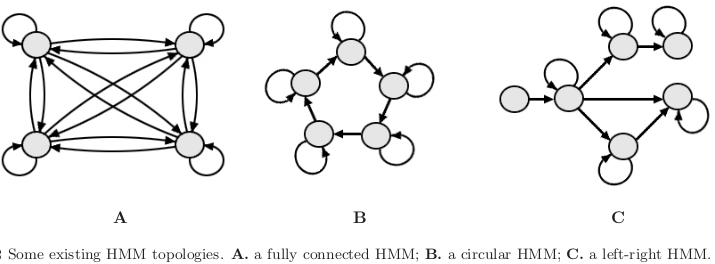
\includegraphics[width = \textwidth]{ChooHMMTopologies.png}
    \caption{Examples of different MC topologies. Credit to Choo et al for the figure \cite{Choo2004}.}
    \label{fig:ChooTopologies}
\end{figure}

\subsection{Hidden Markov Models} \label{Section:HiddenMarkovModels}
Yoon gives a very nice first introduction to Hidden Markov models (HMMs): "A hidden Markov model (HMM) is a statistical model that can be used to describe the evolution of observable events that depend on internal factors, which are not directly observable." \cite{Yoon2009}. A HMM, simply put, is a model that comprises of two different parts. The first part is the sequence or the result that can be observed. A possible observed sequence could be a sequence of nucleotides or it could be a chain of events, like 20 dice throws in a row. The second part is a MC, which is \textit{hidden}, i.e. it cannot be observed. This very simple idea gives a very flexible model, which can be used for many different types of problems. The main goal is often to infer the characteristics of the hidden MC from the observed sequence. 

In a HMM, a hidden sequence of states is generated, according to the MC. This sequence will not be observable and will in (almost) all practical cases be considered as unknown. Each of the states creates, or \textit{emits}, an observed value. All these observed values are what make up the observed sequence. The emission follows a multinomial distribution, where each state follows such a distribution with different parameters. An important assumption for the HMM we will deal with is that the parameters of each multinomial only depends on the state to which it belongs \cite{Choo2004}. This means that the emitted value only depends on its respective hidden state and not on other hidden states. A HMM thus represents a doubly stochastic process: the current underlying state in the MC is stochastic, with an added layer of stochasticity in the observed value. Note that each of the hidden states should be able to produce the same symbols, i.e. the same observable values, but in different frequencies \cite{Christianini2006}.

Following the same notation as earlier, let $\mathbf{X}$ be the random vector that represents the underlying MC of length $L+1$, let $\mathcal{T}$ be the transition probability matrix, let $\mathcal{H}$ denote the hidden states, where $m = \text{card}(\mathcal{H})$, and let $\pi$ be the initial distribution of states. In addition to this, we need to define some notation for the observable sequence in the HMM. First of all, let the random vector $\mathbf{Y} = (Y_0, Y_1, \ldots, Y_L)^T$ represent an observable sequence of length $L+1$. As earlier, $\mathbf{y} = (y_0, y_1, \ldots, y_L)^T$ will represent a realization of $\mathbf{Y}$. Note that both the hidden and the observed sequence are of length $L+1$, since it is assumed that each state emits exactly one symbol. The \textit{symbol alphabet}, i.e. the set of symbols that can be emitted from each state, will be denoted by $\mathcal{S} = \{s_1, \ldots, s_M\}$, where $M = \text{card}(\mathcal{S})$. The \textit{emission probabilities}, i.e. the probabilities used in each multinomial distribution in each state, are usually arranged in a matrix as well. Denote by $\mathcal{E}$ the emission probability matrix. $\mathcal{E}$ is of dimension $m \times M$, where each row in the matrix contains the emission probabilities (of each of the symbols) for a given state. Written in mathematical terms 
\begin{align*}
    \mathcal{E}_{ij} &= \text{P}(Y_t = j|X_t = i), \hspace{0.5em} i \in \mathcal{H}, j \in \mathcal{S}.
\end{align*}
Time-homogeneity is also assumed in the stochastic process of emission, which means that these emission probabilities are the same $\forall t \in [0, L]$. 

A HMM is completely specified by $\pi$, $\mathcal{T}$ and $\mathcal{E}$, where the state space $\mathcal{H}$ and the symbol space $\mathcal{S}$ are indirectly determined by the other quantities \cite{Eddy04}. Once these quantities are specified, one can make calculations concerning the HMM. As already noted, calculating the probability of a given realization $\mathbf{x}$ is 

\begin{equation}
    \text{P}(\mathbf{X} = \mathbf{x}) = \pi(x_0)\prod_{t=2}^L\mathcal{T}_{x_{t-1}, x_t}.
    \label{ProbHiddenMC}
\end{equation}
In a similar fashion, the assumption of independence between states when generating symbols makes it possible to find the probability of the observed sequence simply by taking the product of all appropriate emission probabilities. In mathematical terms, the probability of seeing the sequence $\mathbf{y}$, given the state sequence $\mathbf{x}$, is 

\begin{equation}
    \text{P}(\mathbf{Y} = \mathbf{y}|\mathbf{X}= \mathbf{x}) = \prod_{t=1}^L\mathcal{E}_{x_t, y_t}.
    \label{ProdObservableSeq}
\end{equation}
Finally, combining these results, the joint probability of the sequences $\mathbf{x}$ and $\mathbf{y}$ is 

\begin{equation}
    \text{P}(\mathbf{X} = \mathbf{x}, \mathbf{Y}= \mathbf{y}) = \text{P}(\mathbf{X}= \mathbf{x})\text{P}(\mathbf{Y}= \mathbf{y}|\mathbf{X}= \mathbf{x}) = \pi(x_0)\mathcal{E}_{x_0, y_0}\prod_{t=2}^L\mathcal{E}_{x_t, y_t}\mathcal{T}_{x_{t-1}, x_t}.
    \label{JointProbSequences}
\end{equation}
Keep in mind that the products in equations \eqref{ProbHiddenMC}, \eqref{ProdObservableSeq} and \eqref{JointProbSequences} usually become very small in practice. This can give numerical instability when computing the probabilities. A common trick to solve this is to work with the logarithm of the probabilities. In this way, the multiplicative properties become additive, which mitigates some problems that may occur in the calculations. This is especially important when implementing the algorithms that will be discussed later \cite{Christianini2006}. 

Note that we here assume that the hidden state sequence $\mathbf{x}$ is known, which is usually not the case in practice. The state sequence needs to be inferred from the observed sequence, which is one of the main problems of a HMM, which will be explained in the following. For a more rigorous treatment of this topic, although in the topic of speech recognition, the reader is referred to \cite{Rabiner1989}.


\subsection{Basic Problems for HMMs}
As Yoon \cite{Yoon2009} and Rabiner \cite{Rabiner1989} point out in their respective articles, there are three issues that need to be resolved in order to be able to use HMMs in practical applications. In the following, these issues will be presented, together with algorithms that are used to address the problems. 

A given HMM will in the following be denoted by $\theta = (\pi, \mathcal{T}, \mathcal{E})$. This means that when we refer to a HMM $\theta$, this means that the HMM is fully specified by the three parameters and that the parameters are known. Moreover, for ease of notation, $\text{P}(\mathbf{Y} = \mathbf{y})$ will be denoted as simply $\text{P}(\mathbf{y})$ in the following. 

\subsubsection{The Evaluation Problem}
The first issue that needs to be addressed is: how can the probability $\text{P}(\mathbf{y}|\theta)$ be calculated? That is, how can one find the probability of observing the realization $\mathbf{y}$ from a given HMM $\theta$? If the exact underlying state sequence was known, this would have been easily calculated using equation \eqref{JointProbSequences}. However, the underlying state sequence cannot be observed, which means that there may exist many different underlying state sequences that can yield the same observed sequence $\mathbf{y}$. Thus, the first solution that comes to mind would be to use the law of total probability to calculate

\begin{equation}
    \text{P}(\textbf{y}|\theta) = \sum_{\forall\textbf{x}_i \in \mathcal{H}^n} \text{P}(\textbf{y}, \textbf{x}_i|\theta) = \sum_{\forall\textbf{x}_i \in \mathcal{H}^n} \text{P}(\mathbf{x}_i|\theta)\text{P}(\mathbf{y}|\mathbf{x}_i,\theta), 
\label{unfeasibleForward}
\end{equation}
where $\mathcal{H}^n$ is the space of all possible state sequences that can yield $\mathbf{y}$. Of course, $\mathcal{H}^n$ can be very large, which makes this calculation computationally infeasible. In fact, $\mathcal{H}^n$ may consist of $m^L$ sequences, since these are all the possible state sequences. Luckily, the \textit{forward algorithm} exists, which uses dynamic programming to solve this issue in a computationally feasible manner. This algorithm has time complexity $\mathcal{O}(Lm^2)$, which is a significant improvement over the exponential solution by straightforward use of equation \eqref{unfeasibleForward}. The forward algorithm is given below.  

\begin{algorithm}
    \caption{Forward Algorithm}\label{alg:Forward}
    \begin{algorithmic}
        \STATE $V \gets \text{array}((m+1) \times (L+1))$
        \FOR{$i = 0, 1, \ldots, m$}
            \STATE $V(i,0) \gets \pi(h_{i}) \mathcal{E}_{h_{i},y_0}$
        \ENDFOR
        \FOR{$i = 1, 2, \ldots, L$}
            \FOR{$j = 0,1,\ldots,m$}
                \STATE $V(j,i) \gets \mathcal{E}_{h_{j}, y_i}\sum_{k=0}^{m}V(k, i-1)\mathcal{T}_{h_{k},h_{j}} $
            \ENDFOR
        \ENDFOR
        \RETURN $\text{P}(\mathbf{y}|\theta) \gets \sum_{k=0}^{m}V(k,L)$
    \end{algorithmic} 
\end{algorithm}

Note that the forward algorithm gives a \textit{confidence measure} on the observed sequence - how confident are we that the observed sequence could have been generated by the model $\theta$. This problem is also sometimes referred to as the \textit{scoring problem}, since $\text{P}(\mathbf{y}|\theta)$ is a way to score a new observed sequence based on the given HMM \cite{Yoon2009}. If the calculated probability is lower then some "background distribution" of similar sequences, then the probability of the sequence being emitted by the HMM is low and one would conclude that the HMM is not a good model for the observed sequence. However, if the probability is high, then we can conclude that the HMM can be used in the situation. When this is verified, we tackle the \textit{decoding problem}.

\subsubsection{The Decoding Problem}
The second issue that needs to be addressed is: what state path $\mathbf{x}$ maximizes the probability of emitting the observed sequence $\mathbf{y}$, i.e. how can the \textit{optimal state path} be found? This follows the principle of maximum likelihood, which says that we should choose the hidden state path that maximizes the likelihood of yielding the observed sequence. Our best bet when trying to infer the hidden state path from the observed sequence is exactly the one that gives the maximum probability of obtaining the observed sequence. In other words, the hidden state sequence that best explains the observed sequence is the optimal state path

\begin{equation}
    \mathbf{x^*} = \argmax_\mathbf{X} \text{P}(\mathbf{X}|\mathbf{y}, \theta).
    \label{optimalStatePath}
\end{equation}
Notice that this is equivalent to finding the state sequence that maximizes $\text{P}(\mathbf{X}, \mathbf{y}|\theta)$, because of the definition of conditional probability  

\begin{equation*}
    \text{P}(\mathbf{X}|\mathbf{y}, \theta) = \frac{\text{P}(\mathbf{X}, \mathbf{y}|\theta)}{\text{P}(\mathbf{y}|\theta)}.
\end{equation*}
Again, the first solution that comes to mind would be to compare all possible state sequences $m^L$, and use equation \eqref{JointProbSequences}, but this is still computationally infeasible in most cases. Therefore, the \textit{Viterbi algorithm}, which also is based on dynamic programming, exists. The time complexity of the Viterbi algorithm is $\mathcal{O}(Lm^2)$, which is the same as for the forward algorithm. This is a large improvement over the exponential time-complexity of the straightforward solution. The Viterbi algorithm is given below. 

\begin{algorithm}
\caption{Viterbi Algorithm}\label{alg:Viterbi}
\begin{algorithmic}
    \STATE $V \gets \text{array}((m+1) \times (L+1))$
    \STATE $P \gets \text{array}((m+1) \times (L+1))$
    \FOR{$i = 0, 1, \ldots, m$}
        \STATE $V(i,0) \gets \pi(h_i) \mathcal{E}_{h_i,y_0}$
        \STATE $P(i,0) \gets -1$
    \ENDFOR
    \FOR{$i = 1, 2, \ldots, L$}
        \FOR{$j = 0,1,\ldots,m$}
            \STATE $V(j,i) \gets \mathcal{E}_{h_j, y_i}\max_{k=0,1,\ldots,m}\{V(k, i-1)\mathcal{T}_{h_k,h_j}\}$
            \STATE $P(j,i) \gets \argmax_{k=0,1,\ldots,m}\{V(k, i-1)\mathcal{T}_{h_k,h_j}\mathcal{E}_{h_j, y_i}\}$
        \ENDFOR
    \ENDFOR
    \RETURN $\text{P}(\mathbf{X}|\mathbf{y},\theta) \gets \max_{k=0,1,\ldots,m}V(k,L); \hspace{0.5em}x_L^* = \argmax_{k=0,1,\ldots,m}V(k,L)$
\end{algorithmic} 
\end{algorithm} 
Note that $\mathbf{x}^*$ is simple to find based on $x_L^*$; the optimal path $\mathbf{x}^*$ starts at $x_L^*$ and backtracks all the way to $x_0^*$ by using $P(\cdot, \cdot)$. The backtracking ends when the value $-1$ is found in $P$, i.e. when the beginning of the sequence has been reached. 

Also notice that both the forward and the Viterbi algorithms can easily be $\log$-transformed in order to gain greater numerical stability, by taking logarithms of all values and switching multiplications with additions. 

An important point to make before moving forward is that both the evaluation problem and the decoding problem are related to whether or not an observed sequence can be reasonably modeled by means of a given HMM $\theta$. But how can this model be found in the first place? This is what is often referred to as the \textit{training problem}, which will be covered next. 

\begin{comment}
\textcolor{red}{CAN write about the backward algorithm if time and if it seems relevant. }
The \textit{Backward algorithm} is an alternative ?? The backward algorithm seems like an alternative to the forward algorithm; if the largest probability is known (already found with Viterbi), then it seems like the path that correspond to this probability can be found with the backward algorithm. 

The Viterbi algorithm finds the optimal path for obtaining the entire sequence, i.e. it finds the sequence that maximizes the joint probability of obtaining the entire observed sequence. In some cases, one might be interested in finding the path that gives the largest probability of observing each symbol of the sequence individually. This can be done using the \textit{backward algorithm}. The problem here is to find the state $h_j$ that has the highest likelihood of being the hidden state of $x_j$, i.e. 

\begin{equation*}
    \hat{h}_j = \argmax_i\text{P}(h_j = i|\textbf{X}).
\end{equation*}
As before, searching all the possible states is not a viable option, which is why the backward algorithm is used. It works as ... \textcolor{red}{Continue... Reading from Yoon2009.}

But why do we care about finding the sequence of individually optimal states? This will maximize the expected number of correctly predicted states \cite{Yoon2009} \textcolor{blue}{Hvorfor det egentlig?} Well, if this is the case, why does one even bother using the Viterbi algorithm? The problem with the sequence that maximizes the probability of each observation individually is that it in general will be suboptimal, i.e. that there exists some other sequence $\mathbf{h}^*$ such that $\text{P}(\mathbf{X}, h_1h_2\ldots h_n) \leq \text{P}(\mathbf{X}, \mathbf{h}^*)$. Moreover, the sequence may not even be a possible path for the structure of the HMM, for example if some of the transitions in the predicted sequence are not possible with the given state transition probabilities of the model. For this reason, the Viterbi algorithm is preferred when our goal is to find the optimal path for the entire sequence, while the backward algorithm is preferred when our goal is to infer which state is optimal in a specific position in the sequence. Moreover, the backward algorithm can be used to conclude about the confidence of a state prediction \textcolor{red}{Continue... Reading from Yoon2009.}
\end{comment}

\subsubsection{The Training Problem} \label{Section:TrainingProblem}
The third issue that needs to be addressed is: how can the HMM parameters be reasonably chosen based on a set of observed sequences? For example, we have a set of sequences $\mathbf{\chi} = \{\mathbf{y}_1, \ldots, \mathbf{y}_G\}$, where each $\mathbf{y}_i, \hspace{0.2em} i \in [1,G]$ is an observed sequence of symbols, that we want to represent with a HMM. The difficulty that needs to be solved is how the parameters of the HMM can be estimated based on the set $\mathbf{\chi}$. This is what is typically called the \textit{training} or \textit{learning} problem, analogously to the need for training any other machine learning model. There exists no optimal way to train the HMM from a limited number of finite observation sequences, but there exists algorithms that can find local maximums in the observation probability. Some examples are the Baum-Welch algorithm, standard gradient based methods from optimization or simulation with Monte Carlo expectation maximization (MCEM) \cite{Yoon2009}. For detailed treatments of how the training prblem can be solved, the reader is referred to \cite{Rabiner1989}, \cite{Isaev2006} or \cite{Durbin1998}.

\subsection{HMM Variants}
There exists many variants of what we will call the standard HMM. For completeness, the standard HMM will be specified first, before the most widely used types of HMMs in bioinformatics will be presented. Note that this list is by noe means exhaustive. 

\begin{comment}
\subsubsection{Generalized HMMs}
\textcolor{red}{Changes the distribution of time until state transition (to another state) from geometric to another generalized distribution. Let's see if I have to add it here (depending on if it is used in some of the applicatins in biology. I think this is a continuous time Markov Chain (with sojourn times etc) as learned in StokMod, but not sure. } 
\end{comment}

\subsubsection{Standard HMM}\label{Section:StandardHMM}
The \textit{standard HMM} is the simplest form of a HMM, which has the most restricting assumptions. In fact, the assumptions described in section \ref{Section:HiddenMarkovModels} all belong to what we will call the standard HMM. Concisely restated, the hidden MC is a discrete-state time-homogeneous first-order MC. Also, often one assumes that the MC is \textit{ergodic}, which means that every state can be reached from any other state in a finite amount of states \cite{Rabiner1989}. Moreover, each state in $\mathcal{H}$ generates exactly one output and can emit every symbol in $\mathcal{S}$. Importantly, the emitted value from each states depends only on that respective state. 

All the assumptions made in the simple model restricts the usefulness of the HMM. For example, standard HMMs do not deal well with correlations between residues, since they assume that each residue depends only on one underlying state \cite{Eddy04}. Since the Markov property is assumed, an HMM has no way of "remembering" any distant correlation between the symbols in $\mathcal{S}$. Moreover, Choo et. al writes that "the linear nature of HMM also makes it difficult to capture higher-level information or correlations among amino acids" \cite{Choo2004}. These are only some examples of how restricted the standard HMMs are. 

Despite the fact that the strong assumptions of the standard HMM restrict the flexibility of the model, one can only imagine how the assumptions can be tweaked to create a new type of HMM. Some examples of how changes in the assumptions can mitigate some om the problems of the standard HMM are shown next.  

\subsubsection{Profile-HMM}\label{Section:Profile-HMM}
\textit{Profile-HMM}s (pro-HMMs) have specific architectures, which make them suitable for modeling sequence profiles \cite{Yoon2009}. Because of this, in the context of bioinformatics, the topology of pro-HMMs are best explained with multiple sequence alignment in mind. Two simple ways to think of a pro-HMM is as an abstract description of a protein family or a statistical summary of multiple sequence alignment \cite{Christianini2006}. A pro-HMM is constructed to not contain any cycles. Moreover, a pro-HMM consists of three different types of hidden states: match states ($M_k$), insert states ($I_k$) and delete states ($D_k$). These are used to describe symbol frequencies, insertions and deletions, respectively, at each specific position in a sequence. A great example on how to build a pro-HMM, which helps to clarify the ideas, can be found in \cite{Yoon2009}. The illustration from the example is shown in \ref{fig:Yoon2009ProfileHMMExample}.

\begin{figure}[h]
    \centering
    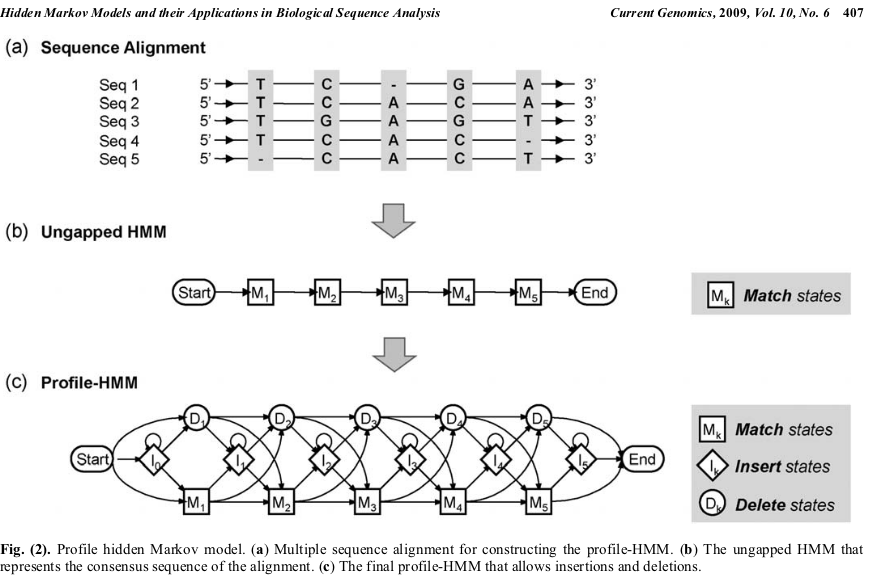
\includegraphics[width = \textwidth]{exampleProfileHMM.png}
    \caption{Figure accompanying the example on how to build a pro-HMM. Credit to Yoon for the figure and the example \cite{Yoon2009}.}
    \label{fig:Yoon2009ProfileHMMExample}
\end{figure}

The example shows how a pro-HMM can be built from a multiple sequence alignment. The idea is that the pro-HMM can be used as a profile to classify new observations; either the new observation fits into the family of sequences that have been aligned, or it does not fit and should be aligned with some other profile. The $M_k$'s are used to indicate match states, i.e. they represent the case where a symbol in a new observation matches with the state of the pro-HMM. The emission probabilities from each match state are easily estimated by using the frequencies of each symbol in the match state. The ungapped HMM can represent ungapped sequences. The states $I_k$ and $D_k$ are added so that the HMM can represent sequences that contain gaps, which makes the pro-HMM a much more powerful model compared to the simpler models that describe a multiple sequence alignment, like regular expressions and PSSM, which we will come back to in section \ref{Section:Motivs}. It is important to note that the delete states $D_k$ are silent states; they are placeholders for missing symbols in the consensus sequence of the alignment when compared to a shorter new observed sequence. 

Note that the pro-HMM parameters can be set in two different ways \cite{Eddy1998}; The first option is to set the parameters from a pre-aligned set of sequences, simply by counting state transitions and emissions, before converting the counts to probabilities. This is how the parameters in the previous example would be set. The second option is to use a set of sequences that is not aligned before training the pro-HMM. This problem is thus analogous to running a multiple sequence alignment before building the model. In this case, algorithms mentioned in section \ref{Section:TrainingProblem} are used. Since these algorithms are only local optimizers it is always advisable to build HMMs on pre-aligned data when this is possible \cite{Eddy1998}. 

\subsubsection{Pair-HMM}
In the context of bioinformatics, a \textit{pair-HMM} (p-HMM) is especially useful for finding sequence alignments and evaluating the significance of the alignments \cite{Yoon2009}. To contrast the standard HMM, a p-HMM generates an aligned pair of sequences, instead of only one sequence. An example is shown in \cite{Yoon2009}, with the illustration from the example shown in figure \ref{fig:Yoon2009PairHMMExample}. The example presents a very simple p-HMM, with hidden states $I_x$, $I_z$ and $A$. This hidden MC produces the two observed sequences denoted by $\mathbf{x}$ and $\mathbf{z}$, where $I_x$ emits an unaligned symbol in sequence $\mathbf{x}$ and $I_z$ emits an unaligned symbol in $\mathbf{z}$. Additionally, state $A$ generates an aligned pair of two symbols, i.e. it inserts two identical symbols, each inserted into each of the observed sequences.  

\begin{figure}[h]
    \centering
    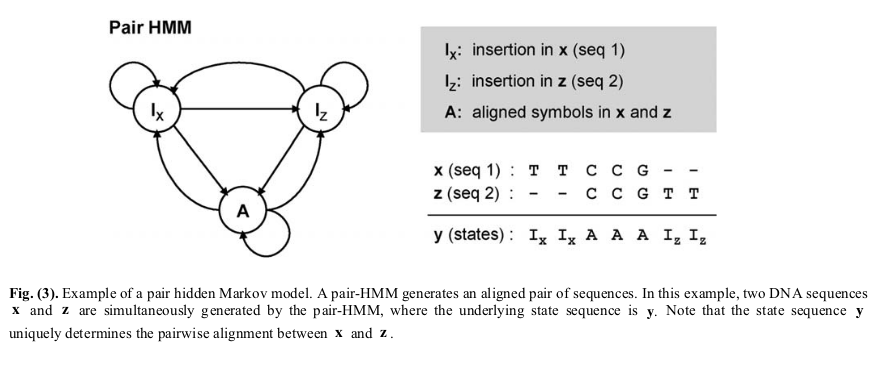
\includegraphics[width = \textwidth]{examplePairHMMYoon.png}
    \caption{Figure accompanying the example on how to build a p-HMM. Credit to Yoon for the figure and the example \cite{Yoon2009}.}
    \label{fig:Yoon2009PairHMMExample}
\end{figure}

Since there is a one-to-one relationship between a hidden state sequence $\mathbf{x}$ of a p-HMM and the alignment between two observed sequences, the alignment problem reduces to finding the optimal state path in the hidden MC. This can be found by a simple variation of the Viterbi algorithm and has time complexity $\mathcal{O}(L_\mathbf{a}L_\mathbf{b})$, where $\mathbf{a}, \mathbf{b}$ are the two sequences that are aligned and $L_\mathbf{a}, L_\mathbf{b}$ are their respective lengths. The p-HMM model is an improvement over the classical sequence alignment methods, since it can be used to compute the alignment probability of the pair of sequences indepently of a specific alignment. A problem in the classical methods is how one should choose a punctuation scheme in order to find a biologically meaningful optimal alignment of the sequences. In cases where this is difficult to choose, it is more meaningful to compute the probability that the sequences are related, which a p-HMM makes possible \cite{Yoon2009}. This probability can be calculated by a slight modification of the forward algorithm. The improvement that a p-HMM gives with respect to pairwise sequence alignment will be further discussed in section \ref{Section:PairwiseSequenceAlignment}.

\subsubsection{Context-Sensitive HMM}\label{Section:cs-HMMs}
As noted in section \ref{Section:StandardHMM}, the standard HMM cannot properly model correlations between residues, which makes the model unsuitable for several applications in biology, for example when dealing with RNA sequences \cite{Yoon2009}. In order to apply the HMM-methodology successfully to such situations, one needs to extend the standard HMM to allow for pairwise correlations between non-adjacent symbols in the observed sequence. This is where the \textit{context-sensitive HMM}s (cs-HMMs) are appropriately applied.

The main difference between cs-HMMs and the standard HMMs is that the former can use information about earlier emissions to adjust the emission probabilities at future states. This information is referred to as the "context". Thus, it is possible to model correlation between non-adjacent states in a cs-HMM. These HMMs use three different types of states: single-emission states ($S_i$),  pairwise-emission states ($P_i$) and context-sensitive states ($C_i$). $S_i$ are very similar to the normal states in ordinary HMMs, since they have usual emission probabilities and do not use any additional information for emitting symbols. $P_i$ have fixed emission probabilities as well, and, in addition, they store the symbols that are admitted in memory. $C_i$ first retrieves the emitted symbol from $P_i$, before adjusting its emission probabilities based on this retrieved context. Thus, we can state the emission probability for this context-sensitive state as 

\begin{equation*}
    \text{P}(y_j|y_k, x_k, x_j) = \text{P}(y_j\text{ emitted at }x_j\text{ given that }y_k\text{ was emitted at }x_k), \hspace{0.5em} j>k
\end{equation*}
where $y_j$ is the emitted symbol at a context-sensitive state $x_j$, $y_k$ is the emitted symbol at a pairwise-emission state $x_k$ and $j>k$, i.e. the MC transitions to the context-sensitive state some time after the pairwise-emission state. Using the fact that $y_k$ is independent of $x_j$, the joint emission probability of $y_k$ and $y_j$ can be calculated

\begin{equation}
    \text{P}(y_k, y_j|x_k, x_j) = \text{P}(y_k|x_k)\text{P}(y_j|y_k, x_k, x_j) = \mathcal{E}_{x_k, y_k}\text{P}(y_j|y_k, x_k, x_j).
    \label{eq:cs-HMMsJointProb}
\end{equation}
Thus, using pairs of states ($P_i, C_i$) allow modeling of pairwise symbol correlation by specifying the emission probabilities that appear in equation \eqref{eq:cs-HMMsJointProb}. Notice that these two states always exist in pairs, since $P_i$ are needed to describe the emission probabilities at $C_i$. Moreover, the model is built such that it is never possible to transition to a context-sensitive state before transitioning to the corresponding pairwise-emission state \cite{Yoon2009}. 

A simple example of a cs-HMM, which is a modified version of an example appearing in \cite{Yoon2009}, is given in figure \ref{fig:Yoon2009ContextSensitiveHMMExample}. The model has three different states: $S_1$ is the only single-emission state, $P_1$ is the only pairwise-emission state and $C_1$ is the only context-sensitive state. The MC first transitions to $P_1$ and emits one or more symbols which are stored in a queue. Note that the figure shows a stack, but in our modified example we are in fact using a queue. Why it matters will hopefully become clear shortly. When the MC eventually transitions to $C_1$, a symbol is retrieved from the queue and the emission probabilities in $C_1$ are adjusted in such a way that the same symbol is emitted. Moreover, in this model, the transition probabilities are adjusted such that the MC transitions only to $C_1$ as long as the queue is not empty. When the queue is empty, the MC transitions to the end state and the simulation is over. Thus, this simple example can be used to create repeating sequences of two different formats. Firstly, the sequence 

\begin{equation*}
    \mathbf{y} = (y_1, y_2, \ldots, y_{(L+1)/2}, y_1, y_2, \ldots, y_{(L+1)/2})^T, 
\end{equation*}
of even length $L+1$ can be generated by the model. In this case, the first $(L+1)/2$ underlying states are $P_1$ and the next $(L+1)/2$ are $C_1$. Secondly, the sequence 

\begin{equation*}
    \mathbf{y} = (y_1, y_2, \ldots, y_{L/2}, y_0, y_1, y_2, \ldots, y_{L/2})^T,
\end{equation*}
of odd length $L+1$ can be generated by the model. In this case, the first $L/2$ underlying states are $P_1$, the underlying state for the $L/2 + 1$ emitted symbol $y_0$ is $S_1$ and the underlying states for the last $y_{L/2}$ are $C_1$. Notice that changing the FIFO queue for a LIFO stack enables generation of  palindromes instead of repeating sequences from the model, as explained in the example by Yoon \cite{Yoon2009}. 

\begin{figure}[h]
    \centering
    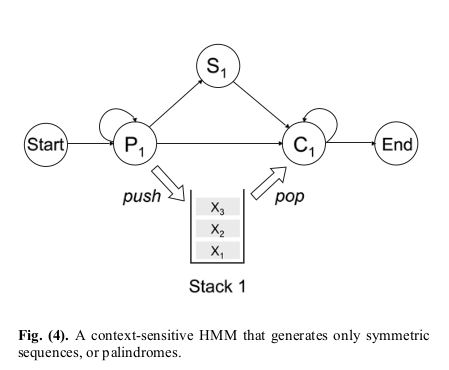
\includegraphics[width = 0.8\textwidth]{ExampleYooncsHMM.png}
    \caption{Figure accompanying the example on how to build a simple cs-HMM. Credit to Yoon for the figure and the example \cite{Yoon2009}. Note that the queue depicted in the figure is changed for a stack in the described example, which changes the generated symbol sequence slightly.}
    \label{fig:Yoon2009ContextSensitiveHMMExample}
\end{figure}

\begin{figure}[h]
    \centering
    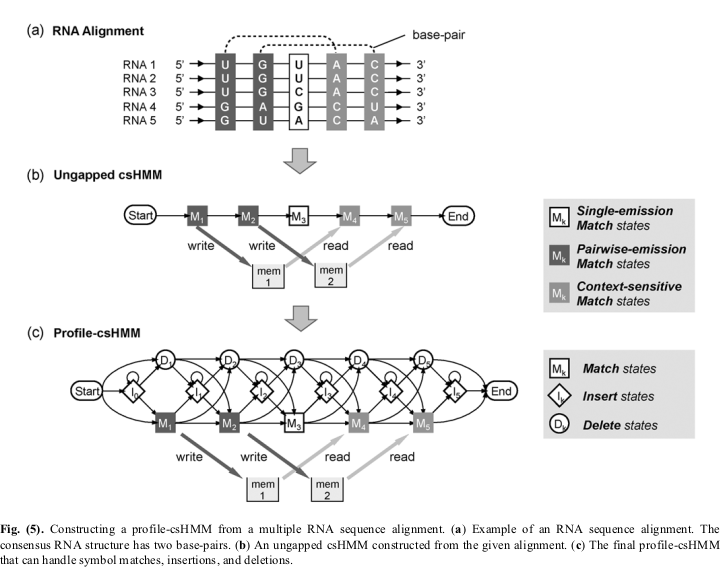
\includegraphics[width = \textwidth]{contextSensHMMExampleYoon.png}
    \caption{Figure accompanying the example on how to build a pro-cs-HMM. Credit to Yoon for the figure and the example \cite{Yoon2009}}
    \label{fig:Yoon2009ProfileContextSensitiveHMMExample}
\end{figure}

Recall that pro-HMMs were used to make profiles that represent multiple alignments of sequences, which in the context of biology can be DNA or proteins. Imagine that we want to make profiles that take column-wise correlations in the multiple alignment into account. This can be done relatively easily by combining the ideas of the pro-HMMs and the cs-HMMs, into what is called \textit{Profile Context-Sensitive HMM}s (pro-cs-HMMs). Like for the pro-HMMs studied earlier, the pro-cs-HMMs contain match states ($M_k$), insert states ($I_k$) and delete states ($D_k$). The new addition to the model is that the match states can be of three different types ($S_i^m, P_i^m, C_i^m$), to account for symbols that are pairwise correlated. The single-emission match states $S_i^m$ are used to represent columns in the multiple alignment that are uncorrelated with the others, while the pairing of ($P_i^m, C_i^m$) are used to model pairwise correlation between symbols in different columns. An example, taken from \cite{Yoon2009}, is shown in figure \ref{fig:Yoon2009ProfileContextSensitiveHMMExample}. The example treats construction of a pro-cs-HMM from the RNA alignment shown in part (a) of the figure. Pairwise emission states are used for columns one and two, while corresponding context-sensitive states are used for columns four and five respectively, in order to model the pairwise correlation between the base-pairs. The third column is simply modelled with a single-emission match state. Thus, part (b) of the figure shows how an ungapped cs-HMM can be constructed. By adding insertion and deletion states, as described in section \ref{Section:Profile-HMM}, the final pro-cs-HMM is constructed. 

For a more detailed treatment of cs-HMMs, the reader is referred to \cite{Yoon2006}.

\section{Applications in Bioinformatics}

\subsection{Pairwise Sequence Alignment}\label{Section:PairwiseSequenceAlignment}
Pairwise sequence alignment (PSA) is carried out in order to infer functional, structural and/or evolutionary relationships between two sequences. Such an alignment can be done both locally and globally and there exists a variety of methods of doing it. Optimal algorithms exist, such as the Needleman-Wunsch algorithm for optimal global alignment and the Smith-Waterman algorithm for optimal local alignment. These algorithms are based on dynamic programming and can be time consuming to use. Therefore, algorithms based on heuristics were developed, where the two most popular algorithms are called BLAST and FASTA. All the mentioned algorithms work well for highly similar sequences, but produce mediocre results for highly divergent sequences \cite{Choo2004}. Profile based analysis was developed to improve these results, in which HMMs play a crucial role. 

A big issue when it comes to finding the best alignment between sequences using the previously mentioned algorithms is that one has to define a reasonable scoring scheme for ranking the possible alignments. It can be difficult to define this scoring scheme, since different scoring schemes perform better or worse in different applications, depending on how similar the sequences are. Thus, the major drawback of these algorithms is the dependence on the scoring scheme, which to a large degree dictates how the alignment is produced, which in turn limits what type of relationship one is able to find between sequences. The p-HMMs introduce an alternative method of finding relationships between a pair of sequences, which distances itself from ad-hoc scoring schemes. 

When using p-HMMs the pairwise sequence alignment problem is tackled as a stochastic process, as used by Smith et al \cite{Smith2003} and Durbin et al \cite{Durbin1998}. Because the p-HMM generates pairs of observations, it can be used to calculate the relationship between two sequences independent of a specific alignment, simply by using the forward algorithm \cite{Choo2004}. A more detailed treatment on how the p-HMMs are used in practice for local and global PSA can be found in Chapter 4 in \cite{Durbin1998}. The bottomline is that p-HMMs give a more general method of PSA compared to the previously mentioned algorithms, because the parameters $\theta$ of the HMM can be estimated, as discussed in the training problem, instead of having to manually define a scoring scheme that makes biological sense in the specific problem. For a more detailed treatment of PSA, the reader is referred to \cite{Durbin1998}.

This section only discusses PSA in the context of sequences of nucleotides or aminoacids, i.e. PSA of DNA sequences or proteins. Alignment of RNA sequences can become more complex, which will be shortly discussed in section \ref{RNAStructuralAlignment}.

\subsection{Multiple Sequence Alignment}\label{Section:MSA}
Multiple sequence alignment (MSA) is commonly used to find conserved regions in a group of sequences and predicting protein structures. Functional biological sequences typically come in families, which means that one is interested in discovering possible relationships between a sequence and a known sequence family. Despite the fact that sequences will have diverged from each other in evolution, MSA can be used to identify which sequences belong to a family, in order to allow for inferences about their function \cite{Durbin1998}. This application of MSA will be studied further in sections \ref{Section:ProtHomoDetect} and \ref{Section:ProtPredFunc}. Moreover, MSA is interesting in the case of protein structure prediction, because one can align structural data instead of sequences \cite{Eddy1998}. This application of MSA will be further discussed in section \ref{Section:ProtStructurePred}. 

In contrast to PSA, there does not exist any optimal algorithms to solve the multiple alignment problem. However, there exists a variety of heuristic methods for solving it. One possible solution is to reduce the multiple alignment problem to a set of pairwise comparisons between the sequences, in an orderly fashion, in order to end up with the multiple alignment in the end. Here one can choose to use either the optimal algorithms or the heuristic algorithms when performing the pairwise alignment. One type of methods that employs this paradigm is referred to as \textit{progressive sequence alignment}. More details on a progressive algorithm that uses Needleman-Wunsch for the pairwise alignment can be found in \cite{Feng1987}. Some commonly available implementations of this solution include the T-Coffee and the Clustal package \cite{EMBL-EBI-Multiple}. Another type of methods that uses this paradigm is referred to as \textit{iterative alignment}. These methods are slightly different from the progressive methods, since they allow re-alignment of the pairwise sequences during multiple iterations. The progressive methods do not facilitate this, which means that they depend highly on the initial pairwise alignment of the first two sequences \cite{BioInfoOrgMSA}. One popular openly available implementation of an iterative method is MUSCLE \cite{EMBL-EBI-Multiple}. 

As in the case of PSA, HMMs provide powerful alternatives to the mentioned methods for MSA. In this problem, pro-HMMs have been particularly successful. Choo et al states that "Multiple alignments from a group of unaligned sequences are automatically created using the Viterbi algorithm" \cite{Choo2004}. Each match state in the pro-HMM corresponds to to a column in the MSA. We refer back to section \ref{Section:Profile-HMM} for a brief description of how the pro-HMM relates to MSA. 

The beaty of a pro-HMM in the case of MSA is that they can be treated as a summary of a multiple alignment of sequences or as a model for a family of such sequences \cite{Christianini2006}. These pro-HMM representations of MSAs make it possible to use the MSA for many different applications in biology. They facilitate quick assignment of protein function, based on alignment of a new sequence against the model. Moreover, a pro-HMM that represents a family of sequences can be used to search for homologues. The model can be used to search in a database of sequences, in order to find additional homologues to the family. Similarly, given a database of pre-built pro-HMMs, one can look for matching profiles to a symbol sequence. Thus, such a database can be used to classify and annotate the given sequence. Additionally, pro-HMMs can be used to compare two different MSAs. This can be beneficial for detecting remote homologues \cite{Yoon2009}. Thus, the pro-HMM representation of a MSA is very flexible, as it can be applied to many different problems by following different principles. Once a pro-HMM is constructed one can align new sequences to it, one can use it to query in databases of sequences, one can query a database of such pro-HMMs for matching profiles to one symbol sequence or one can compare two different pro-HMMs in order to discover similarities between two different MSAs. 

Finally, we mention two free online repositories that store pre-built pro-HMMs of many known protein families: PFAM and PROSITE. 

For a more detailed treatment of MSA, the reader is referred to \cite{Durbin1998}.

\subsection{Motif Representation}\label{Section:Motivs}
A motif is a recurring pattern in DNA or proteins, which is assumed to be related to biological function. Thus a motif can be a sequence of nucleotides or of aminoacids. Finding such motifs is interesting to a biologist because \textit{transcription factor binding sites} (TFBS) appear as such motifs in sequences. These are regulatory sequences that control gene transcription, which is important information for a biologist because they repress or promote the expression of many other genes \cite{Christianini2006}.

There are several ways of representing such sequence motifs, where the performance of each method generally depends on what type of motifs one wants to represent. For shorter, ungapped motifs of fixed length, methods like \textit{consensus sequences}, \textit{regular expressions} (RegEx), \textit{sequence logos} and \textit{position specific scoring matrix} (PSSM), in ascending order of complexity, are commonly used. Note that these can also be seen as different ways of visualizing or representing MSAs, which are useful tools in practice, since the alignments themselves are not very easy in use. 

The drawbacks of these methods are that they do not work well for longer motifs with variable length gaps. This is where pro-HMMs shine in comparison. The HMMs work well for all types of motifs, including the short and fixed length motifs, but they are more complicated models. Thus, even though the HMMs always will produce good results, given that they can be built correctly in each specific case, one should not always use these models because of their complexity. Always keep the principle of parsimony in mind; for competing explanations, or models, where all are reasonable, one should always choose the simplest, which meakes the least amount of assumptions. Hence, even though the HMMs are great tools also for motif representation, they should be used when appropriate. 

But how can the HMMs be used to represent motifs with variable length gaps? pro-HMMs have gained much traction for this problem, since they yield very reliable results. How they work can be seen easily from the example presented about the pro-HMMs in section \ref{Section:Profile-HMM}, since the example shows how a MSA can be represented as a pro-HMM. The same principle explained in the example can be used when working with much larger and more complicated alignments. As you have noted by now, motif representation is very closely related to MSA, which means that the tactics used for querying with pro-HMMs described in section \ref{Section:MSA} also apply here. 

Note that the problem of indentifying the motifs is not discussed in detail here, as this is a much more complicated problem compared to simply representing the motifs. However, this problem is similar to multiple local alignment. An example of an algorithm to solve this problem is given in chapter 10.3 in \cite{Christianini2006}, which is a variant of the Gibbs sampling algorithm based on PSSMs. 

\subsection{Protein Homology Detection}\label{Section:ProtHomoDetect}
Protein homology detection concerns the problem of discovering homologous proteins, i.e. which proteins are derived from a common ancestor. This knowledge plays a very important role in the study of protein structures and function. A scientist wants to characterize sets of homologous proteins (gene families) based on common patterns in their sequence. Once such a characterization is found from a known family, one can determine if a new protein belongs to this family or not \cite{Christianini2006}. The attentive reader will notice that this simply can be seen as an application of sequence alignment. 

The methods that perhaps first come to mind for solving this problem are the methods for PSA first mentioned in \ref{Section:PairwiseSequenceAlignment} and for MSA in \ref{Section:MSA}. An interesting with more details about how these methods are used for homology detection is \cite{Pearson2013}. Other methods for solving this problem relies on more modern and more sophisticated machine learning models than HMMs, as for example the employment of Bidirectional Long Short-Term Memory (BLSTM) and neural networks \cite{Li2017}. This shows a recurring theme in bioinformatics; new models are developed, some of which outperform older models, while others cannot compete. Several examples of such developments will be described in other applications later on as well. 

When treating this as an application of MSA it is readily seen that this type of homology detection can be done with pro-HMMs. As noted by Christianini and Hahn in \textit{Introduction to Computational Genomics} "profile HMMs encode position-specific information about the frequency of particular amino acids as well as the frequency of insertions and deletions in the alignment. They are constructed from multiple alignments
of homologous sequences" \cite{Christianini2006}. Thus, aligning a sequence with a pro-HHM is equivalent to aligning the sequence to many other sequences, which where used to establish the pro-HMM in the first place. The pro-HMM can be used to query a database of sequences or a database of other pro-HMMs in order to find additional homologues. 

Remote protein homology detection can be more complicated, which means that the standard pro-HMMs can be unreliable. To improve the performance of pro-HMMs in such cases, models known as \textit{feature-based profile-HMMs} can be used. More information about these models can be found in \cite{Yoon2009}. Distant homologous relationships between proteins can for example also be detected based on pairwise alignment of pro-HMMs, as noted in section \ref{Section:MSA}. One such method can be found in \cite{Soding2005}.

\subsection{Prediction of Function}\label{Section:ProtPredFunc}
Probably the most important characteristic of a protein is its function, which is not inherently known, unless it already has been discovered. This means that, given a specific protein with unknown function, a scientist is interested in predicting its function. One way of making this prediction possible is the attempt of inferring functional similarity between a given protein, with unknown function, and a protein with previously discovered function. But how can this similarity be inferred? 

As noted in section \ref{Section:MSA}, functional biological sequences typically come in families. This assumption makes it possible to infer functional similarity based on similarities in the sequences of proteins. The attentive reader will notice that this can be solved via sequence alignment as well. The simplest possible solution could be to compare the protein with unknown function pairwise, sequentially, to a database of proteins with known functions. This can be time-consuming and inaccurate however, since PSA does not guarantee finding similarity between the sequences. This is because sequences that are evolutionary related can differ a lot, i.e. not be very similar, but still have the same function. Such sequences would get a low score in the PSA. To mitigate such problems, MSA is more widely used, because of the familiarity assumption. Thus, having built a pro-HMM from a family of proteins with known function, this model can be used to infer whether or not a new protein shares the same function. Searching an extensive database of pre-built pro-HMMs one can (hopefully) find what function a specific protein most likely possesses. Notice that this problem is very closely related to protein homology detection, as described earlier. 

\subsection{Protein Structure Prediction}\label{Section:ProtStructurePred}
Another important characteristic of a protein is its structure. The structure of a protein provides "a key to understanding its biological function" \cite{Isaev2006}. Generally, the structure of a protein can be distinguished into four different levels; primary, secondary, tertiary and quaternary. Without going into closer details about what the different levels mean, each of them describe different characteristics of the protein's structure, where the primary structure is the aminoacid sequence itself. The main goal of structure prediction is to predict the secondary, tertiary and quaternary levels from the primary level of a specific protein. This is interesting because the experimental approaches used to discover all the structural levels of a protein are expensive, difficult and time-consuming. Because of these difficulties, the ideal is to use computational and statistical models to predict unknown structures. However, note that the idea of predicting all levels from the primary level is very optimistic in most cases. In practice, one can only hope to predict the secondary structure, and sometimes the tertiary structure, as noted by Isaev \cite{Isaev2006}.

One set of widely used models for predicting the secondary structure of a protein are pro-HMMs. This problem can, again, be seen as an application of MSA. When searching for a particular structural feature in a protein with unknown structure, one constructs a pro-HMM from a set of proteins with this feature. Then, aligning the query sequence to the pro-HMM can decide whether or not the sequence in question has the structural feature. In practice, one would query a database of pro-HMMs constructed based on different structural features, in order to (hopefully) uncover one of the features in the query protein.  

For prediction of the tertiary structure of a protein, one possible methodology is described by Yoon \cite{Yoon2009}. He notes that pro-HMMs can be used to "model sequences of protein secondary structure symbols: helix (H), strand (E) and coil (C)" \cite{Yoon2009}. Such models can be used to recognize the three-dimensional fold of new protein sequences based on their secondary protein structure predictions. Thus, this methodology assumes the secondary structure of the protein as known, either from experimental approaches or prediction. 

Despite the vast improvements the HMMs have yielded, Eddy notes that "Profile HMMs and HMM-based gene finders have probably been the most successful applications of HMMs in computational biology. On the other hand, protein secondary structure prediction is an area in which the state of the art is neural net methods that outperform HMM methods by using extensive local correlation information that is not necessarily easy to model in an HMM" \cite{Eddy1998}. This shows that the HMMs that are used up until now are not the be-all and end-all for statistical methods in bioinformatics, and that today's most successful method may be surpassed in the future. 

More details about this problem, which is also known as the \textit{protein folding problem}, can be found in Isaev's \textit{Introduction to Mathematical Methods in Bioinformatics} \cite{Isaev2006}. A more technical note can be found in \cite{Choo2004}. Again, notice that this problem is very closely related to protein homology detection, as described earlier. 

\subsection{Segmentation}
Segmentation is about defining exact boundaries between distinct regions with different chemical properties. Moreover, segmentation is about defining larger sequences of heterogeneous nucleotide in genome and to identify biological features that are responsible for the heterogeneity that is observed \cite{Christianini2006}. 

HMMs can be used effectively for segmentation as well. Some important points when using HMMs for segmentation; the hidden states of a HMM are interpreted as different types of the sequence and the hidden alphabet is typically very small. The underlying MC is cyclic in this case, allowing returns to the same state, i.e. to the same type of sequence, many times during the simulation \cite{Christianini2006}. Example 4.2 in Christianini and Hahn's \textit{Introduction to Computational Genomics} shows a simple genomic segmentation using HMMs. In fact, this example is very similar to the example that will be presented in section \ref{Section:ToyExample}, which is about building a simple HMM for the cleavage of a DNA sequence between areas rich in CG or AT. 

\subsection{Gene Prediction}
Gene prediction refers to the problem of identifying regions of genomic DNA that encode genes. Also known as \textit{gene finding} this was largely based on experimentation earlier, but in later times it has been transformed to a largely computational problem. It seems like most of the computational methods that are used to solve this problem are based on HMMs. An article by Scalzitti et al from 2020 references five widely used gene prediction programs, where all are based on HMMs \cite{Scalzitti2020}.

HMMs can be employed to find eukaryotic genes and to find pseudogenes, which look like functioning genes except for some misplaced stop codons. They are very useful models for these problems because of their flexibility \cite{Christianini2006}. Moreover, as discussed by Yoon, p-HMMs can be used for gene prediction \cite{Yoon2009}. Additionally, extensions of the HMM that are not mentioned in this report, that are called \textit{generalized HMMs} and \textit{generalized p-HMMs} can be used for gene prediction and genomic annotation \cite{Choo2004} \cite{Yoon2009}. Lastly, an overview of some more methods that have been used for gene prediction can be found in \cite{Sleator2010}.

\subsection{RNA Structural Alignment}\label{RNAStructuralAlignment}
Instead of aligning protein sequences to predict structure, as explained in section \ref{Section:ProtStructurePred}, this problem is about aligning structural data tied to RNA. This can be more complicated because, as Yoon notes, "due to the conservation of seconday structure, multiple RNA alignments often display column-wise correlation" \cite{Yoon2009}.

As explained in section \ref{Section:cs-HMMs}, pro-cs-HMMs can be used to represent RNA alignments. However, pro-cs-HMMs can also perform structural alignment of RNA, as well as similarity searches, analagously to how the pro-HMMs can be used to perform multiple alignment of DNA or proteins and to perform similarity searches in these cases. RNA sequence analysis is often of high computational complexity, because the alignment algorithms have to deal with base-pair correlations in the sequences that may be very complicated. More details about this problem in \cite{Yoon2009}.

As a sidenote, p-HMMs on tree structures (PHHMTS) can be used for aligning trees. Since most RNA secondary structures can be represented as trees, this provides a useful framework for aligning RNA sequences. More details can be found in \cite{Sakakibara2003}.

\subsection{Other Applications}
Some more applications of HMMs, all described by Yoon, are \textit{base-calling}, \textit{modeling DNA sequencing errors} and \textit{mcRNA indentification} \cite{Yoon2009}. These are all interesting problems, but will not be described here. 

Either way, based on the short list of applications that have been described, it has hopefully become clear to the reader that HMMs are very widely used in Bioinformatics. 

\section{Examples in R}

\subsection{Toy Example}\label{Section:ToyExample}

Simple HMMs can relatively easily be programmed manually. Imagine that you want to build a simple HMM for the cleavage of a DNA sequence between areas rich in CG or AT. The HMM would take the form as depicted in figure \ref{fig:toy_hmm}. The hidden MC has two states ($AT$ and $CG$), where $AT$ represents an $AT$ rich state and CG represents a CG rich state. In mathematical terms, we would write that $\mathcal{H} = \{AT, CG\}$. Moreover, since we are working with sequences of DNA, $\mathcal{S} = \{A,C,G,T\}$. The transition probabilities and the emission probabilities are shown in figure \ref{fig:toy_hmm}. Note that the initial state probabilities are omitted from the figure, but they are set in the simulated model below. Based on these probabilities, the matrices are

\begin{equation*}
  \mathcal{T} = \begin{bmatrix}
      \mathcal{T}_{AT, AT} & \mathcal{T}_{AT, CG} \\
      \mathcal{T}_{CG, AT} & \mathcal{T}_{CG, CG}  \\
  \end{bmatrix} = \mathcal{T} = \begin{bmatrix}
      0.8 & 0.2 \\
      0.2 & 0.8  \\
  \end{bmatrix},
\end{equation*}
and 
\begin{equation*}
  \mathcal{E} = \begin{bmatrix}
      \mathcal{E}_{AT, A} & \mathcal{E}_{AT, C} & \mathcal{E}_{AT, G} & \mathcal{E}_{AT, T}\\
      \mathcal{E}_{CG, A} & \mathcal{E}_{CG, C} & \mathcal{E}_{CG, G} & \mathcal{E}_{CG, T}\\
  \end{bmatrix} = \begin{bmatrix}
     0.4 & 0.1 & 0.1 & 0.4 \\
      0.1 & 0.4 & 0.4 & 0.1 \\
  \end{bmatrix}.
\end{equation*}

\tikzstyle{startend}=[shape=circle,draw=black, very thick, minimum size=0.5cm]
\tikzstyle{state}=[shape=circle,draw=black, very thick, minimum size=1cm]
\tikzstyle{observation}=[shape=rectangle,draw=orange!50,fill=orange!20]
\tikzstyle{lightedge}=[<-,dotted]
\tikzstyle{mainstate}=[state,thick]
\tikzstyle{mainedge}=[<-,thick]

\begin{figure}[htbp]
    \begin{center}
    \begin{tikzpicture}[every left delimiter/.style={xshift=1ex}]
        
        % states
        \node[state] (s1) at (3.33,0) {$AT$};
        \node[state] (s3) at (6.66,0) {$CG$};
    
        %loopback prob labels
        \node[below = 0.25cm of s1, inner sep=0pt, outer sep = 0pt, minimum size = 25pt]
                (s1loopback) {0.8};
        \node[below = 0.25cm of s3, inner sep=0pt, outer sep = 0pt, minimum size = 25pt]
                (s3loopback) {0.8};
    
        %emission probabilities
        \node[align=center, above left = 1cm and -1cm of s1, blue] (emit1) {
            \(
            \begin{cases}
                A = 0.4 \\
                C = 0.1 \\
                G = 0.1 \\
                T = 0.4
            \end{cases}
            \)
        };
        \node[align=center, above right = 1cm and -1cm of s3, blue] (emit3) {
            \(
            \begin{cases}
                A = 0.1 \\
                C = 0.4 \\
                G = 0.4 \\
                T = 0.1
            \end{cases}
            \)
        };
                
        %all edges
        \path[]
            
            (s1) edge [-{>[scale=1]}, out=30, in=150, thick, midway, above] node {0.2} (s3)
            
            (s3) edge [-{>[scale=1]}, out = 210, in = 330, thick, midway, above] node {0.2} (s1)
    
            %  Loop back edges
            (s1) edge [thick, out=300, in=0] (s1loopback)
            (s1loopback) edge [thick, -{>[scale=1]}, out=180, in=240] (s1)
            (s3) edge [thick, out=300, in=0] (s3loopback)
            (s3loopback) edge [thick, -{>[scale=1]}, out=180, in=240] (s3)
            
            
            %   Connect emission probs
            (emit1) edge [thick, blue, out=225, in=135] (s1)
            (emit3) edge [thick, blue, out=315, in=45] (s3);
    
    \end{tikzpicture}
    \end{center}
    \caption{HMM topology for example on modelling the cleavage of a DNA sequence between areas rich in CG or AT. Note that the initial state probabilites are omitted from this figure. }
    \label{fig:toy_hmm}
\end{figure}


The code block below shows one simple example of how this example HMM can be simulated. The function takes four inputs; the transition matrix, the emission matrix, the length of sequence that one wants to simulate and the initial state probabilities. 

\begin{knitrout}
\definecolor{shadecolor}{rgb}{0.969, 0.969, 0.969}\color{fgcolor}\begin{kframe}
\begin{alltt}
\hlstd{generate.sequences} \hlkwb{<-} \hlkwa{function}\hlstd{(}\hlkwc{Tr}\hlstd{,} \hlkwc{Em}\hlstd{,} \hlkwc{n}\hlstd{,} \hlkwc{p}\hlstd{)\{}
    \hlcom{# Tr = transition matrix.}
    \hlcom{# Em = emission matrix.}
    \hlcom{# n = length of generated sequence.}
    \hlcom{# p = initial state probabilities. }

  \hlstd{symbols} \hlkwb{<-} \hlkwd{c}\hlstd{(}\hlstr{"A"}\hlstd{,} \hlstr{"C"}\hlstd{,} \hlstr{"G"}\hlstd{,} \hlstr{"T"}\hlstd{)}
  \hlstd{states} \hlkwb{<-} \hlkwd{c}\hlstd{(}\hlnum{1}\hlstd{,} \hlnum{2}\hlstd{)} \hlcom{# 1 = AT and 2 = CG}

  \hlcom{# x are hidden states and y are observed symbols. }
  \hlstd{x} \hlkwb{<-} \hlstd{y} \hlkwb{<-} \hlkwd{rep}\hlstd{(}\hlnum{NA}\hlstd{,} \hlkwc{length.out} \hlstd{= n)}

  \hlstd{x[}\hlnum{1}\hlstd{]} \hlkwb{<-} \hlkwd{sample}\hlstd{(states,} \hlkwc{size} \hlstd{=} \hlnum{1}\hlstd{,} \hlkwc{prob} \hlstd{= p)}
  \hlstd{y[}\hlnum{1}\hlstd{]} \hlkwb{<-} \hlkwd{sample}\hlstd{(symbols,} \hlkwc{size} \hlstd{=} \hlnum{1}\hlstd{,}\hlkwc{replace}\hlstd{=T,}\hlkwc{prob} \hlstd{= Em[x[}\hlnum{1}\hlstd{],])}

  \hlkwa{for}\hlstd{(i} \hlkwa{in} \hlnum{1}\hlopt{:}\hlstd{(n}\hlopt{-}\hlnum{1}\hlstd{))\{}
    \hlstd{x[i}\hlopt{+}\hlnum{1}\hlstd{]} \hlkwb{<-} \hlkwd{sample}\hlstd{(states,} \hlkwc{size} \hlstd{=} \hlnum{1}\hlstd{,} \hlkwc{prob} \hlstd{= Tr[,x[i]])}
    \hlstd{y[i}\hlopt{+}\hlnum{1}\hlstd{]} \hlkwb{<-} \hlkwd{sample}\hlstd{(symbols,} \hlkwc{size} \hlstd{=} \hlnum{1}\hlstd{,} \hlkwc{prob} \hlstd{= Em[x[i], ])}
  \hlstd{\}}
  \hlkwd{return}\hlstd{(}\hlkwd{cbind}\hlstd{(}\hlstr{"Hidden"} \hlstd{= x,} \hlstr{"Obs"} \hlstd{= y))}
\hlstd{\}}
\end{alltt}
\end{kframe}
\end{knitrout}

For example, the code block below shows how a HMM of length $n = 1000$, according to the specifications listed above, can be simulated, using the function `generate.sequences`.

\begin{knitrout}
\definecolor{shadecolor}{rgb}{0.969, 0.969, 0.969}\color{fgcolor}\begin{kframe}
\begin{alltt}
\hlcom{# Transition matrix (A).}
\hlstd{A} \hlkwb{<-} \hlkwd{matrix}\hlstd{(}\hlkwd{c}\hlstd{(}\hlnum{0.8}\hlstd{,} \hlnum{0.2}\hlstd{,} \hlnum{0.2}\hlstd{,} \hlnum{0.8}\hlstd{),} \hlkwc{nrow} \hlstd{=} \hlnum{2}\hlstd{)}
\hlkwd{rownames}\hlstd{(A)} \hlkwb{<-} \hlkwd{c}\hlstd{(}\hlstr{"AT"}\hlstd{,} \hlstr{"CG"}\hlstd{)}
\hlkwd{colnames}\hlstd{(A)} \hlkwb{<-} \hlkwd{c}\hlstd{(}\hlstr{"AT"}\hlstd{,} \hlstr{"CG"}\hlstd{)}
\hlstd{A}
\end{alltt}
\begin{verbatim}
##     AT  CG
## AT 0.8 0.2
## CG 0.2 0.8
\end{verbatim}
\begin{alltt}
\hlcom{# Emission matrix (E).}
\hlstd{E} \hlkwb{<-} \hlkwd{matrix}\hlstd{(}\hlkwd{c}\hlstd{(}\hlnum{0.4}\hlstd{,} \hlnum{0.1}\hlstd{,} \hlnum{0.1}\hlstd{,} \hlnum{0.4}\hlstd{,} \hlnum{0.1}\hlstd{,} \hlnum{0.4}\hlstd{,} \hlnum{0.4}\hlstd{,} \hlnum{0.1}\hlstd{),} \hlkwc{nrow} \hlstd{=} \hlnum{2}\hlstd{)}
\hlkwd{rownames}\hlstd{(E)} \hlkwb{<-} \hlkwd{c}\hlstd{(}\hlstr{"AT"}\hlstd{,} \hlstr{"CG"}\hlstd{)}
\hlkwd{colnames}\hlstd{(E)} \hlkwb{<-} \hlkwd{c}\hlstd{(}\hlstr{"A"}\hlstd{,} \hlstr{"C"}\hlstd{,} \hlstr{"G"}\hlstd{,} \hlstr{"T"}\hlstd{)}
\hlstd{E}
\end{alltt}
\begin{verbatim}
##      A   C   G   T
## AT 0.4 0.1 0.1 0.4
## CG 0.1 0.4 0.4 0.1
\end{verbatim}
\begin{alltt}
\hlcom{# Initial probabilities.}
\hlstd{p} \hlkwb{<-} \hlkwd{c}\hlstd{(}\hlnum{0.2}\hlstd{,}\hlnum{0.8}\hlstd{)}

\hlcom{# Length of the sequence.}
\hlstd{n} \hlkwb{<-} \hlnum{1000}

\hlcom{# Generate the sequences. }
\hlkwd{set.seed}\hlstd{(}\hlnum{1234}\hlstd{)}
\hlstd{df} \hlkwb{<-} \hlkwd{generate.sequences}\hlstd{(A, E, n, p)}

\hlcom{# The first 5 steps in the chains is printed below. }
\hlstd{df[}\hlnum{1}\hlopt{:}\hlnum{5}\hlstd{, ]}
\end{alltt}
\begin{verbatim}
##      Hidden Obs
## [1,] "2"    "G"
## [2,] "2"    "G"
## [3,] "1"    "G"
## [4,] "1"    "A"
## [5,] "1"    "T"
\end{verbatim}
\end{kframe}
\end{knitrout}


Chapter 10.6 in \cite{Krijnen2009} is a good reference for some more simple manual implementations of MCs and HMMs in R. Although it is always recommended to try to implement methods manually at first, because it helps to understand the theory to a greater degree, the use of libraries always gives more flexibility. Moreover, libraries are very often optimized, such that the performance and reliability of the code is guaranteed. We will be diving deeper into one such library for HMMs in R in the following. 

\subsection{The \textit{aphid} Library}

The \textit{aphid} library in R was "designed for the development and application of hidden Markov models and profile HMMs for biological sequence analysis", as the author states in the package description in the \textit{Comprehensive R Archive Network} (CRAN) \cite{CRAN}. There exists a great vignette for the package, written by the author of \textit{aphid}  himself, which we will be following to some degree here \cite{Wilkinson2017}. It contains several examples of how the package can be used, as well as descriptions of exactly what it contains. As will be shown, the library even has plotting capabilites, i.e. it can plot a diagram, similar to the one seen in figure \ref{fig:toy_hmm}, representing the HMM in a particular case. For more information, or if anything is unclear, consult this vignette and the documentation of the library. 

\subsubsection{Fair Bet Casino}
A typical first example of the use of a HMM is the so-called "Fair Bet Casino" \cite{Jones2004}. In this casino, a dealer flips a coin and a player bets on the outcome. The dealer uses either a fair coin, where flipping either heads or tails is equally likely, or a biased coin, where one of the sides is much more likely. For the sake of this demonstration, heads is given the probability $\frac34$. Moreover, the dealer does not like to switch coins very often. In this case, the switch only happens with probability $\frac17$. Moreover, we assume that the dealer starts with the fair coin in 99\% of the games he deals. Given a sequence of coin tosses, the player wants to figure out which of the coins the dealer has used, since this can help the player to win more money. Hopefully it is clear to you that this problem can be modelled as a standard HMM, as introduced in section \ref{Section:StandardHMM}. This can be done in a very simple manner, via the \textit{aphid} library, as shown below.   

\begin{center}
\begin{knitrout}
\definecolor{shadecolor}{rgb}{0.969, 0.969, 0.969}\color{fgcolor}\begin{kframe}
\begin{alltt}
\hlkwd{library}\hlstd{(}\hlstr{"aphid"}\hlstd{)}
\hlstd{states} \hlkwb{<-} \hlkwd{c}\hlstd{(}\hlstr{"Begin"}\hlstd{,} \hlstr{"Fair"}\hlstd{,} \hlstr{"Biased"}\hlstd{)}
\hlstd{symbols} \hlkwb{<-} \hlkwd{c}\hlstd{(}\hlstr{"H"}\hlstd{,} \hlstr{"T"}\hlstd{)}

\hlcom{# Define transition probability matrix A.}
\hlstd{A} \hlkwb{<-} \hlkwd{matrix}\hlstd{(}\hlkwd{c}\hlstd{(}\hlnum{0}\hlstd{,} \hlnum{0}\hlstd{,} \hlnum{0}\hlstd{,} \hlnum{0.99}\hlstd{,} \hlnum{6}\hlopt{/}\hlnum{7}\hlstd{,} \hlnum{1}\hlopt{/}\hlnum{7}\hlstd{,} \hlnum{0.1}\hlstd{,} \hlnum{1}\hlopt{/}\hlnum{7}\hlstd{,} \hlnum{6}\hlopt{/}\hlnum{7}\hlstd{),} \hlkwc{nrow} \hlstd{=} \hlnum{3}\hlstd{)}
\hlkwd{dimnames}\hlstd{(A)} \hlkwb{<-} \hlkwd{list}\hlstd{(}\hlkwc{from} \hlstd{= states,} \hlkwc{to} \hlstd{= states)}
\hlstd{A}
\end{alltt}
\begin{verbatim}
##         to
## from     Begin      Fair    Biased
##   Begin      0 0.9900000 0.1000000
##   Fair       0 0.8571429 0.1428571
##   Biased     0 0.1428571 0.8571429
\end{verbatim}
\begin{alltt}
\hlcom{# Define emission probability matrix E.}
\hlstd{E} \hlkwb{<-} \hlkwd{matrix}\hlstd{(}\hlkwd{c}\hlstd{(}\hlkwd{rep}\hlstd{(}\hlnum{1}\hlopt{/}\hlnum{2}\hlstd{,} \hlnum{2}\hlstd{),} \hlnum{3}\hlopt{/}\hlnum{4}\hlstd{,} \hlnum{1}\hlopt{/}\hlnum{4}\hlstd{),} \hlkwc{nrow} \hlstd{=} \hlnum{2}\hlstd{,} \hlkwc{byrow} \hlstd{=} \hlnum{TRUE}\hlstd{)}
\hlkwd{dimnames}\hlstd{(E)} \hlkwb{<-} \hlkwd{list}\hlstd{(}\hlkwc{states} \hlstd{= states[}\hlopt{-}\hlnum{1}\hlstd{],} \hlkwc{symbols} \hlstd{= symbols)}
\hlstd{E}
\end{alltt}
\begin{verbatim}
##         symbols
## states      H    T
##   Fair   0.50 0.50
##   Biased 0.75 0.25
\end{verbatim}
\begin{alltt}
\hlcom{# Create the HMM object.}
\hlstd{x} \hlkwb{<-} \hlkwd{structure}\hlstd{(}\hlkwd{list}\hlstd{(}\hlkwc{A} \hlstd{= A,} \hlkwc{E} \hlstd{= E),} \hlkwc{class} \hlstd{=} \hlstr{"HMM"}\hlstd{)}

\hlcom{# Plot the model.}
\hlkwd{plot}\hlstd{(x,} \hlkwc{textexp} \hlstd{=} \hlnum{1.5}\hlstd{)}

\hlcom{# Optionally add the transition probabilities as text.}
\hlkwd{text}\hlstd{(}\hlkwc{x} \hlstd{=} \hlnum{0.02}\hlstd{,} \hlkwc{y} \hlstd{=} \hlnum{0.5}\hlstd{,} \hlkwc{labels} \hlstd{=} \hlstr{"6/7"}\hlstd{)}
\hlkwd{text}\hlstd{(}\hlkwc{x} \hlstd{=} \hlnum{0.53}\hlstd{,} \hlkwc{y} \hlstd{=} \hlnum{0.5}\hlstd{,} \hlkwc{labels} \hlstd{=} \hlstr{"6/7"}\hlstd{)}
\hlkwd{text}\hlstd{(}\hlkwc{x} \hlstd{=} \hlnum{0.5}\hlstd{,} \hlkwc{y} \hlstd{=} \hlnum{0.3}\hlstd{,} \hlkwc{labels} \hlstd{=} \hlstr{"1/7"}\hlstd{)}
\hlkwd{text}\hlstd{(}\hlkwc{x} \hlstd{=} \hlnum{0.5}\hlstd{,} \hlkwc{y} \hlstd{=} \hlnum{0.7}\hlstd{,} \hlkwc{labels} \hlstd{=} \hlstr{"1/7"}\hlstd{)}
\end{alltt}
\end{kframe}
\includegraphics[width=\maxwidth]{figure/unnamed-chunk-3-1} 
\end{knitrout}
\end{center}

Interestingly, this simple version of the "Fair Bet Casino" can be used to find so-called "CG-islands", which are genomic regions where CG appears frequently compared to other areas in the rest of the genome. The reader is referred to chapter 11 in Jones and Pevzner's \textit{An Introduction to Bioinformatics Algorithms} for an interesting read concerning this example \cite{Jones2004}.

In order to highlight some more of the capabilities of the library, another example of such an imaginary casino will be used, based on chapter 3.2 in Durbin et al \cite{Durbin1998}. This casino has two dice, one fair and one weighted. The fair dice emits each of the six sides with equal probabilites, while the probability of rolling a "6" is $\frac{1}{2}$ for the loaded dice, while the probability of rolling any of the other sides is $\frac{1}{10}$. The dealer switches from the fair dice to the loaded dice with probability $\frac{5}{100}$ and from the loaded dice to the fair dice with probability $\frac{1}{10}$. This situation is modelled with the library in the following block of code. 

\begin{center}
\begin{knitrout}
\definecolor{shadecolor}{rgb}{0.969, 0.969, 0.969}\color{fgcolor}\begin{kframe}
\begin{alltt}
\hlstd{states} \hlkwb{<-} \hlkwd{c}\hlstd{(}\hlstr{"Begin"}\hlstd{,} \hlstr{"Fair"}\hlstd{,} \hlstr{"Loaded"}\hlstd{)}
\hlstd{residues} \hlkwb{<-} \hlkwd{paste}\hlstd{(}\hlnum{1}\hlopt{:}\hlnum{6}\hlstd{)}

\hlcom{# Define transition probability matrix A.}
\hlstd{A} \hlkwb{<-} \hlkwd{matrix}\hlstd{(}\hlkwd{c}\hlstd{(}\hlnum{0}\hlstd{,} \hlnum{0}\hlstd{,} \hlnum{0}\hlstd{,} \hlnum{0.99}\hlstd{,} \hlnum{0.95}\hlstd{,} \hlnum{0.1}\hlstd{,} \hlnum{0.01}\hlstd{,} \hlnum{0.05}\hlstd{,} \hlnum{0.9}\hlstd{),} \hlkwc{nrow} \hlstd{=} \hlnum{3}\hlstd{)}
\hlkwd{dimnames}\hlstd{(A)} \hlkwb{<-} \hlkwd{list}\hlstd{(}\hlkwc{from} \hlstd{= states,} \hlkwc{to} \hlstd{= states)}
\hlstd{A}
\end{alltt}
\begin{verbatim}
##         to
## from     Begin Fair Loaded
##   Begin      0 0.99   0.01
##   Fair       0 0.95   0.05
##   Loaded     0 0.10   0.90
\end{verbatim}
\begin{alltt}
\hlcom{# Define emission probability matrix E.}
\hlstd{E} \hlkwb{<-} \hlkwd{matrix}\hlstd{(}\hlkwd{c}\hlstd{(}\hlkwd{rep}\hlstd{(}\hlnum{1}\hlopt{/}\hlnum{6}\hlstd{,} \hlnum{6}\hlstd{),} \hlkwd{rep}\hlstd{(}\hlnum{1}\hlopt{/}\hlnum{10}\hlstd{,} \hlnum{5}\hlstd{),} \hlnum{1}\hlopt{/}\hlnum{2}\hlstd{),} \hlkwc{nrow} \hlstd{=} \hlnum{2}\hlstd{,} \hlkwc{byrow} \hlstd{=} \hlnum{TRUE}\hlstd{)}
\hlkwd{dimnames}\hlstd{(E)} \hlkwb{<-} \hlkwd{list}\hlstd{(}\hlkwc{states} \hlstd{= states[}\hlopt{-}\hlnum{1}\hlstd{],} \hlkwc{residues} \hlstd{= residues)}
\hlstd{E}
\end{alltt}
\begin{verbatim}
##         residues
## states           1         2         3         4         5         6
##   Fair   0.1666667 0.1666667 0.1666667 0.1666667 0.1666667 0.1666667
##   Loaded 0.1000000 0.1000000 0.1000000 0.1000000 0.1000000 0.5000000
\end{verbatim}
\begin{alltt}
\hlcom{# Create the HMM object.}
\hlstd{x} \hlkwb{<-} \hlkwd{structure}\hlstd{(}\hlkwd{list}\hlstd{(}\hlkwc{A} \hlstd{= A,} \hlkwc{E} \hlstd{= E),} \hlkwc{class} \hlstd{=} \hlstr{"HMM"}\hlstd{)}

\hlcom{# Plot the model.}
\hlkwd{plot}\hlstd{(x,} \hlkwc{textexp} \hlstd{=} \hlnum{1.5}\hlstd{)}

\hlcom{# Optionally add the transition probabilities as text.}
\hlkwd{text}\hlstd{(}\hlkwc{x} \hlstd{=} \hlnum{0.02}\hlstd{,} \hlkwc{y} \hlstd{=} \hlnum{0.5}\hlstd{,} \hlkwc{labels} \hlstd{=} \hlstr{"0.95"}\hlstd{)}
\hlkwd{text}\hlstd{(}\hlkwc{x} \hlstd{=} \hlnum{0.51}\hlstd{,} \hlkwc{y} \hlstd{=} \hlnum{0.5}\hlstd{,} \hlkwc{labels} \hlstd{=} \hlstr{"0.90"}\hlstd{)}
\hlkwd{text}\hlstd{(}\hlkwc{x} \hlstd{=} \hlnum{0.5}\hlstd{,} \hlkwc{y} \hlstd{=} \hlnum{0.9}\hlstd{,} \hlkwc{labels} \hlstd{=} \hlstr{"0.05"}\hlstd{)}
\hlkwd{text}\hlstd{(}\hlkwc{x} \hlstd{=} \hlnum{0.5}\hlstd{,} \hlkwc{y} \hlstd{=} \hlnum{0.1}\hlstd{,} \hlkwc{labels} \hlstd{=} \hlstr{"0.10"}\hlstd{)}
\end{alltt}
\end{kframe}
\includegraphics[width=\maxwidth]{figure/unnamed-chunk-4-1} 
\end{knitrout}
\end{center}

Let us solve the decoding problem for a given observed sequence of dice residuals. The library includes a few data sets, where one of the data sets is called \textit{casino}, which is data taken from this exact example. The data contains the result of 300 rolls of the dice that switched from fair to loaded, i.e. a sequence from the data set contains the hidden MC and the observed sequence of symbols. In the code block below, the hidden MC state sequence is first extracted from the data set. Then the Viterbi algorithm is used to solve the decoding problem, given (only) the observed sequence of symbols from the data set. 

\begin{knitrout}
\definecolor{shadecolor}{rgb}{0.969, 0.969, 0.969}\color{fgcolor}\begin{kframe}
\begin{alltt}
\hlcom{# Load the data set.}
\hlkwd{data}\hlstd{(casino)}

\hlcom{# The actual path is stored in the names attribute of the sequence.}
\hlstd{actual} \hlkwb{<-} \hlkwd{c}\hlstd{(}\hlstr{"F"}\hlstd{,} \hlstr{"L"}\hlstd{)[}\hlkwd{match}\hlstd{(}\hlkwd{names}\hlstd{(casino),} \hlkwd{c}\hlstd{(}\hlstr{"Fair"}\hlstd{,} \hlstr{"Loaded"}\hlstd{))]}

\hlcom{# Find the predicted path.}
\hlstd{vit1} \hlkwb{<-} \hlkwd{Viterbi}\hlstd{(x, casino)}

\hlcom{# vit1 contains several types of information. }
\hlkwd{names}\hlstd{(vit1)}
\end{alltt}
\begin{verbatim}
## [1] "score"   "path"    "array"   "pointer"
\end{verbatim}
\begin{alltt}
\hlcom{# The predicted path from the Viterbi algorithm. }
\hlstd{predicted} \hlkwb{<-} \hlkwd{c}\hlstd{(}\hlstr{"F"}\hlstd{,} \hlstr{"L"}\hlstd{)[vit1}\hlopt{$}\hlstd{path} \hlopt{+} \hlnum{1}\hlstd{]}
\hlcom{# Note the path element of the output Viterbi object is an integer vector.}
\hlcom{# The addition of 1 to the path converts from C/C++ to R's indexing style.}

\hlcom{# Comparing the predicted and the actual path. }
\hlstd{(df} \hlkwb{<-} \hlkwd{rbind}\hlstd{(}\hlkwc{actual} \hlstd{= actual,} \hlkwc{predicted} \hlstd{= predicted))}
\end{alltt}
\begin{verbatim}
##           [,1] [,2] [,3] [,4] [,5] [,6] [,7] [,8] [,9] [,10] [,11] [,12] [,13]
## actual    "F"  "F"  "F"  "F"  "F"  "F"  "F"  "F"  "F"  "F"   "F"   "F"   "F"  
## predicted "F"  "F"  "F"  "F"  "F"  "F"  "F"  "F"  "F"  "F"   "F"   "F"   "F"  
##           [,14] [,15] [,16] [,17] [,18] [,19] [,20] [,21] [,22] [,23] [,24]
## actual    "F"   "F"   "F"   "F"   "F"   "F"   "F"   "F"   "F"   "F"   "F"  
## predicted "F"   "F"   "F"   "F"   "F"   "F"   "F"   "F"   "F"   "F"   "F"  
##           [,25] [,26] [,27] [,28] [,29] [,30] [,31] [,32] [,33] [,34] [,35]
## actual    "F"   "F"   "F"   "F"   "F"   "F"   "F"   "F"   "F"   "F"   "F"  
## predicted "F"   "F"   "F"   "F"   "F"   "F"   "F"   "F"   "F"   "F"   "F"  
##           [,36] [,37] [,38] [,39] [,40] [,41] [,42] [,43] [,44] [,45] [,46]
## actual    "F"   "F"   "F"   "F"   "F"   "F"   "F"   "F"   "F"   "F"   "L"  
## predicted "F"   "F"   "F"   "F"   "F"   "F"   "F"   "F"   "F"   "F"   "F"  
##           [,47] [,48] [,49] [,50] [,51] [,52] [,53] [,54] [,55] [,56] [,57]
## actual    "L"   "L"   "L"   "L"   "L"   "L"   "L"   "L"   "L"   "L"   "L"  
## predicted "F"   "F"   "L"   "L"   "L"   "L"   "L"   "L"   "L"   "L"   "L"  
##           [,58] [,59] [,60] [,61] [,62] [,63] [,64] [,65] [,66] [,67] [,68]
## actual    "L"   "L"   "L"   "L"   "L"   "L"   "L"   "L"   "L"   "F"   "F"  
## predicted "L"   "L"   "L"   "L"   "L"   "L"   "L"   "L"   "L"   "F"   "F"  
##           [,69] [,70] [,71] [,72] [,73] [,74] [,75] [,76] [,77] [,78] [,79]
## actual    "F"   "F"   "F"   "F"   "F"   "F"   "F"   "F"   "F"   "F"   "L"  
## predicted "F"   "F"   "F"   "F"   "F"   "F"   "F"   "F"   "F"   "F"   "L"  
##           [,80] [,81] [,82] [,83] [,84] [,85] [,86] [,87] [,88] [,89] [,90]
## actual    "L"   "L"   "L"   "L"   "L"   "L"   "L"   "L"   "L"   "L"   "L"  
## predicted "L"   "L"   "L"   "L"   "L"   "L"   "L"   "L"   "L"   "L"   "L"  
##           [,91] [,92] [,93] [,94] [,95] [,96] [,97] [,98] [,99] [,100] [,101]
## actual    "L"   "L"   "L"   "L"   "F"   "F"   "F"   "L"   "L"   "L"    "L"   
## predicted "L"   "L"   "L"   "L"   "L"   "L"   "L"   "L"   "L"   "L"    "L"   
##           [,102] [,103] [,104] [,105] [,106] [,107] [,108] [,109] [,110] [,111]
## actual    "L"    "L"    "L"    "L"    "L"    "L"    "L"    "L"    "L"    "L"   
## predicted "L"    "L"    "L"    "L"    "L"    "L"    "L"    "L"    "L"    "L"   
##           [,112] [,113] [,114] [,115] [,116] [,117] [,118] [,119] [,120] [,121]
## actual    "F"    "F"    "F"    "F"    "F"    "F"    "F"    "F"    "F"    "F"   
## predicted "L"    "F"    "F"    "F"    "F"    "F"    "F"    "F"    "F"    "F"   
##           [,122] [,123] [,124] [,125] [,126] [,127] [,128] [,129] [,130] [,131]
## actual    "F"    "F"    "F"    "F"    "F"    "F"    "F"    "L"    "L"    "L"   
## predicted "F"    "F"    "F"    "F"    "F"    "F"    "F"    "F"    "F"    "F"   
##           [,132] [,133] [,134] [,135] [,136] [,137] [,138] [,139] [,140] [,141]
## actual    "L"    "L"    "L"    "L"    "L"    "L"    "L"    "L"    "L"    "L"   
## predicted "F"    "F"    "F"    "F"    "F"    "F"    "F"    "F"    "F"    "F"   
##           [,142] [,143] [,144] [,145] [,146] [,147] [,148] [,149] [,150] [,151]
## actual    "F"    "F"    "F"    "F"    "F"    "F"    "F"    "F"    "F"    "F"   
## predicted "F"    "F"    "F"    "F"    "F"    "F"    "F"    "F"    "F"    "F"   
##           [,152] [,153] [,154] [,155] [,156] [,157] [,158] [,159] [,160] [,161]
## actual    "F"    "F"    "F"    "F"    "F"    "F"    "F"    "F"    "F"    "F"   
## predicted "F"    "F"    "F"    "F"    "F"    "F"    "F"    "F"    "F"    "F"   
##           [,162] [,163] [,164] [,165] [,166] [,167] [,168] [,169] [,170] [,171]
## actual    "F"    "F"    "F"    "F"    "F"    "F"    "F"    "F"    "F"    "F"   
## predicted "F"    "F"    "F"    "F"    "F"    "F"    "F"    "F"    "F"    "F"   
##           [,172] [,173] [,174] [,175] [,176] [,177] [,178] [,179] [,180] [,181]
## actual    "F"    "F"    "F"    "F"    "F"    "F"    "F"    "L"    "L"    "L"   
## predicted "F"    "F"    "F"    "F"    "F"    "F"    "F"    "F"    "L"    "L"   
##           [,182] [,183] [,184] [,185] [,186] [,187] [,188] [,189] [,190] [,191]
## actual    "L"    "L"    "L"    "L"    "L"    "L"    "L"    "F"    "F"    "F"   
## predicted "L"    "L"    "L"    "L"    "L"    "L"    "L"    "L"    "L"    "L"   
##           [,192] [,193] [,194] [,195] [,196] [,197] [,198] [,199] [,200] [,201]
## actual    "F"    "F"    "F"    "F"    "F"    "F"    "F"    "F"    "F"    "F"   
## predicted "L"    "F"    "F"    "F"    "F"    "F"    "F"    "F"    "F"    "F"   
##           [,202] [,203] [,204] [,205] [,206] [,207] [,208] [,209] [,210] [,211]
## actual    "F"    "F"    "F"    "F"    "F"    "F"    "F"    "F"    "F"    "F"   
## predicted "F"    "F"    "F"    "F"    "F"    "F"    "F"    "F"    "F"    "F"   
##           [,212] [,213] [,214] [,215] [,216] [,217] [,218] [,219] [,220] [,221]
## actual    "F"    "F"    "F"    "F"    "F"    "F"    "F"    "F"    "F"    "F"   
## predicted "F"    "F"    "F"    "F"    "F"    "F"    "F"    "F"    "F"    "F"   
##           [,222] [,223] [,224] [,225] [,226] [,227] [,228] [,229] [,230] [,231]
## actual    "F"    "F"    "F"    "F"    "F"    "F"    "F"    "F"    "F"    "F"   
## predicted "F"    "F"    "F"    "F"    "F"    "F"    "F"    "F"    "F"    "F"   
##           [,232] [,233] [,234] [,235] [,236] [,237] [,238] [,239] [,240] [,241]
## actual    "F"    "F"    "F"    "F"    "F"    "F"    "F"    "F"    "F"    "F"   
## predicted "F"    "F"    "F"    "F"    "F"    "F"    "F"    "F"    "F"    "F"   
##           [,242] [,243] [,244] [,245] [,246] [,247] [,248] [,249] [,250] [,251]
## actual    "F"    "F"    "F"    "F"    "F"    "F"    "F"    "F"    "F"    "F"   
## predicted "F"    "F"    "F"    "F"    "F"    "F"    "F"    "F"    "F"    "F"   
##           [,252] [,253] [,254] [,255] [,256] [,257] [,258] [,259] [,260] [,261]
## actual    "F"    "F"    "F"    "F"    "F"    "F"    "F"    "F"    "F"    "F"   
## predicted "F"    "F"    "F"    "F"    "F"    "F"    "F"    "F"    "F"    "F"   
##           [,262] [,263] [,264] [,265] [,266] [,267] [,268] [,269] [,270] [,271]
## actual    "F"    "F"    "F"    "F"    "F"    "F"    "L"    "L"    "L"    "L"   
## predicted "F"    "F"    "F"    "F"    "F"    "F"    "F"    "F"    "F"    "L"   
##           [,272] [,273] [,274] [,275] [,276] [,277] [,278] [,279] [,280] [,281]
## actual    "L"    "L"    "L"    "L"    "L"    "L"    "L"    "L"    "L"    "L"   
## predicted "L"    "L"    "L"    "L"    "L"    "L"    "L"    "L"    "L"    "L"   
##           [,282] [,283] [,284] [,285] [,286] [,287] [,288] [,289] [,290] [,291]
## actual    "L"    "L"    "L"    "L"    "L"    "L"    "L"    "L"    "F"    "F"   
## predicted "L"    "L"    "L"    "L"    "L"    "L"    "L"    "L"    "F"    "F"   
##           [,292] [,293] [,294] [,295] [,296] [,297] [,298] [,299] [,300]
## actual    "F"    "F"    "F"    "F"    "F"    "F"    "F"    "F"    "F"   
## predicted "F"    "F"    "F"    "F"    "F"    "F"    "F"    "F"    "F"
\end{verbatim}
\end{kframe}
\end{knitrout}

The training problem can also be solved using the library. The function used below uses the method described in chapter 3.3 in Durbin et al, which assumes that the state sequences in all the training data is known \cite{Durbin1998}. It derives a standard HMM from the sequence in the data set, which is plotted. 

\begin{center}
\begin{knitrout}
\definecolor{shadecolor}{rgb}{0.969, 0.969, 0.969}\color{fgcolor}\begin{kframe}
\begin{alltt}
\hlstd{y} \hlkwb{<-} \hlkwd{deriveHMM}\hlstd{(}\hlkwd{list}\hlstd{(casino),} \hlkwc{logspace} \hlstd{=} \hlnum{FALSE}\hlstd{)}
\hlkwd{plot}\hlstd{(y,} \hlkwc{textexp} \hlstd{=} \hlnum{1.5}\hlstd{)}

\hlcom{# Optionally add the transition probabilities as text.}
\hlkwd{text}\hlstd{(}\hlkwc{x} \hlstd{=} \hlnum{0.02}\hlstd{,} \hlkwc{y} \hlstd{=} \hlnum{0.5}\hlstd{,} \hlkwc{labels} \hlstd{=} \hlkwd{round}\hlstd{(y}\hlopt{$}\hlstd{A[}\hlstr{"Fair"}\hlstd{,} \hlstr{"Fair"}\hlstd{],} \hlnum{2}\hlstd{))}
\hlkwd{text}\hlstd{(}\hlkwc{x} \hlstd{=} \hlnum{0.51}\hlstd{,} \hlkwc{y} \hlstd{=} \hlnum{0.5}\hlstd{,} \hlkwc{labels} \hlstd{=} \hlkwd{round}\hlstd{(y}\hlopt{$}\hlstd{A[}\hlstr{"Loaded"}\hlstd{,} \hlstr{"Loaded"}\hlstd{],} \hlnum{2}\hlstd{))}
\hlkwd{text}\hlstd{(}\hlkwc{x} \hlstd{=} \hlnum{0.5}\hlstd{,} \hlkwc{y} \hlstd{=} \hlnum{0.9}\hlstd{,} \hlkwc{labels} \hlstd{=} \hlkwd{round}\hlstd{(y}\hlopt{$}\hlstd{A[}\hlstr{"Fair"}\hlstd{,} \hlstr{"Loaded"}\hlstd{],} \hlnum{2}\hlstd{))}
\hlkwd{text}\hlstd{(}\hlkwc{x} \hlstd{=} \hlnum{0.5}\hlstd{,} \hlkwc{y} \hlstd{=} \hlnum{0.1}\hlstd{,} \hlkwc{labels} \hlstd{=} \hlkwd{round}\hlstd{(y}\hlopt{$}\hlstd{A[}\hlstr{"Loaded"}\hlstd{,} \hlstr{"Fair"}\hlstd{],} \hlnum{2}\hlstd{))}
\end{alltt}
\end{kframe}
\includegraphics[width=\maxwidth]{figure/unnamed-chunk-6-1} 
\end{knitrout}
\end{center}

Despite the fact that the function is only fed with one sequence (which is all our data set contains), the parameters of the HMM are estimated relatively closely to the correct model. Usually, we will feed a training algorithm with many more sequences, such that the correct model is more closely mirrored. The library contains more methods for solving the training problem, for both standard HMMs and pro-HMMs, but this is the most simple example. The vignette contains examples on the use of these as well \cite{Wilkinson2017}.

Lastly, how a pro-HMM, as introducted in section \ref{Section:Profile-HMM}, can be derived from a sequence is shown. The library contains another data set called \textit{globins}. This contains small globin alignment data, which is taken from figure 5.3 in Durbin et al \cite{Durbin1998}. This alignment data can be used to build a pro-HMM, as shown below. 

\begin{center}
\begin{knitrout}
\definecolor{shadecolor}{rgb}{0.969, 0.969, 0.969}\color{fgcolor}\begin{kframe}
\begin{alltt}
\hlkwd{data}\hlstd{(globins)}
\hlstd{globins}
\end{alltt}
\begin{verbatim}
##            [,1] [,2] [,3] [,4] [,5] [,6] [,7] [,8] [,9] [,10]
## HBA_HUMAN  "V"  "G"  "A"  "-"  "-"  "H"  "A"  "G"  "E"  "Y"  
## HBB_HUMAN  "V"  "-"  "-"  "-"  "-"  "N"  "V"  "D"  "E"  "V"  
## MYG_PHYCA  "V"  "E"  "A"  "-"  "-"  "D"  "V"  "A"  "G"  "H"  
## GLB3_CHITP "V"  "K"  "G"  "-"  "-"  "-"  "-"  "-"  "-"  "D"  
## GLB5_PETMA "V"  "Y"  "S"  "-"  "-"  "T"  "Y"  "E"  "T"  "S"  
## LGB2_LUPLU "F"  "N"  "A"  "-"  "-"  "N"  "I"  "P"  "K"  "H"  
## GLB1_GLYDI "I"  "A"  "G"  "A"  "D"  "N"  "G"  "A"  "G"  "V"
\end{verbatim}
\begin{alltt}
\hlstd{globins.PHMM} \hlkwb{<-} \hlkwd{derivePHMM}\hlstd{(globins,} \hlkwc{residues} \hlstd{=} \hlstr{"AMINO"}\hlstd{,} \hlkwc{pseudocounts} \hlstd{=} \hlstr{"Laplace"}\hlstd{)}
\end{alltt}
\begin{verbatim}
## Applying uniform sequence weights
\end{verbatim}
\begin{alltt}
\hlkwd{plot}\hlstd{(globins.PHMM)}
\end{alltt}
\end{kframe}
\includegraphics[width=\maxwidth]{figure/unnamed-chunk-7-1} 
\end{knitrout}
\end{center}

\begin{thebibliography}{20}
\bibitem{Eddy04}
Sean R. Eddy (2004) \emph{What is a hidden Markov model?}, Nature Biotechnology, Volume 22, Number 10, 1315-1316.

\bibitem{Choo2004} 
Khar H. Choo, Joo C. Tong, Louxin Zhang (2004) \emph{Recent Applications of Hidden Markov Models in Computational Biology}, Geno. Prot. Bioinfo, Vol. 2, No. 2, 84-96.

\bibitem{Yoon2009}
Byung-Jun Yoon (2009) \emph{Hidden Markov Models and their Applications in Biological Sequence Analysis}, Bentham Science Publishers Ltd., Current Genomics, Vol. 10, No. 6, 402-415.

\bibitem{Christianini2006}
Nello Christianini, Matthew W. Hahn (2006) \emph{Introduction to Computational Genomics: A Case Studies Approach}, Cambridge University Press.

\bibitem{Smith2003}
Smith, L., et al. (2003) \emph{Hidden Markov models and optimized sequence alignments}, Computational Biology and Chemistry, Vol. 27, 77-84.

\bibitem{Feng1987}
Feng DF, Doolittle RF (1987) \emph{Progressive sequence alignment as a prerequisite to correct phylogenetic trees}, J Mol Evol. Vol. 25, No. 4, 351-360. doi: 10.1007/BF02603120. PMID: 3118049.

\bibitem{Pinsky2011}
Mark A. Pinsky, Samuel Karlin (2011) \emph{An Introduction to Stochastic Modeling}, Fourth Edition, Elsevier

\bibitem{EMBL-EBI-Multiple}
EMBL-EBI, \emph{Multiple Sequence Alignment}, downloaded on 03.12.21, 
url: \verb$https://www.ebi.ac.uk/Tools/msa/$

\bibitem{BioInfoOrgMSA}
Bioinformatics Organization, \emph{Multiple sequence alignment}, downloaded on 04.12.21, 
url: \verb$https://www.bioinformatics.org/wiki/Multiple_sequence_alignment$


\bibitem{Rabiner1989}
Lawrence R. Rabiner (1989) \emph{A tutorial on hidden Markov models and selected applications in speech recognition}, Proceedings of the IEEE, Vol. 77, No. 2, 257-286

\bibitem{Isaev2006}
Alexander Isaev (2006) \emph{Introduction to Mathematical Methods in Bioinformatics}, Springer-Verlag

\bibitem{Durbin1998}
R. Durbin, S. Eddy, A. Krogh, G. Mitchison (1998) \emph{Biological Sequence Analysis}, Cambridge University Press

\bibitem{Eddy1998}
Sean R. Eddy (1998) \emph{Profile hidden Markov models}, Bioinformatics Review, Volume 14, Number 9, 755-763.

\bibitem{Yoon2006}
Byung-Jun Yoon, P. P. Vaidyanathan (2006) \emph{Context-Sensitive Hidden Markov Models for Modeling Long-Range Dependencies in Symbol Sequences}, IEEE TRANSACTIONS ON SIGNAL PROCESSING, Volume 54, Number 11, 4169-4184.

\bibitem{Krijnen2009}
Wim P. Krijnen (2009) \emph{Applied Statistics for Bioinformatics using R}, GNU Free Document Licence

\bibitem{CRAN}
CRAN, \emph{aphid: Analysis with Profile Hidden Markov Models}, downloaded on 11.01.22, 
url: \verb$https://CRAN.R-project.org/package=aphid$

\bibitem{Wilkinson2017}
Shaun Wilkinson (2017), \emph{The ‘aphid’ package for analysis with profile hidden Markov models}, downloaded on 11.01.22, 
url: \verb$https://cran.r-project.org/web/packages/aphid/vignettes/aphid-vignette.html$

\bibitem{Jones2004}
Neil C. Jones, Pavel A. Pevzner (2004) \emph{An Introduction to Bioinformatics Algorithms}, MIT Press. 

\bibitem{Li2017}
Li, S., Chen, J. \& Liu, B. (2017) \emph{Protein remote homology detection based on bidirectional long short-term memory}, BMC Bioinformatics 18, 443. \verb$https://doi.org/10.1186/s12859-017-1842-2$

\bibitem{Soding2005}
Johannes Söding (2005) \emph{Protein homology detection by HMM–HMM comparison}, Bioinformatics, Volume 21, Issue 7, 1 April 2005, Pages 951-960. \verb$https://doi.org/10.1093/bioinformatics/bti125$

\bibitem{Pearson2013}
Pearson W. R. (2013) \emph{An introduction to sequence similarity ("homology") searching}. Current protocols in bioinformatics, Chapter 3, Unit3.1. \verb$https://doi.org/10.1002/0471250953.bi0301s42$

\bibitem{Sleator2010}
Roy D. Sleator (2010) \emph{An overview of the current status of eukaryote gene prediction strategies}. Gene, Volume 461, Issues 1-2, Pages1-4. \verb$https://doi.org/10.1016/j.gene.2010.04.008$

\bibitem{Scalzitti2020}
Scalzitti, N., Jeannin-Girardon, A., Collet, P. et al. (2020) \emph{A benchmark study of ab initio gene prediction methods in diverse eukaryotic organisms}. BMC Genomics 21, 293. \verb$https://doi.org/10.1186/s12864-020-6707-9$

\bibitem{Sakakibara2003}
Sakakibara Y. (2003) \emph{Pair hidden Markov models on tree structures}. Bioinformatics, 2003;19 Suppl 1:i232-40. \verb$10.1093/bioinformatics/btg1032$

\end{thebibliography}

\end{document}
